\documentclass[10pt, xcolor=x11names,compress, aspectratio=169]{beamer}
\usepackage{tabulary}
\usepackage{booktabs}
\usepackage{float}
\usepackage{graphicx}
\graphicspath{{../Figures/}}
\usepackage{mwe}% for example pictures
\usepackage{siunitx}
\usepackage{hyperref}
\usepackage{amssymb} 
\usepackage{natbib}
\usepackage{fancyhdr}

\usecolortheme{dolphin}

% set colors
\definecolor{myNewColorA}{RGB}{25,25,112}
\definecolor{myNewColorB}{RGB}{25,25,112}
\definecolor{myNewColorC}{RGB}{25,25,112}
\setbeamercolor*{palette primary}{bg=myNewColorC}
\setbeamercolor*{palette secondary}{bg=myNewColorB, fg = white}
\setbeamercolor*{palette tertiary}{bg=myNewColorA, fg = white}
\setbeamercolor*{titlelike}{fg=myNewColorA}
\setbeamercolor*{title}{bg=myNewColorA, fg = white}
\setbeamercolor*{item}{fg=myNewColorA}
\setbeamercolor*{caption name}{fg=myNewColorA}
\usefonttheme{professionalfonts}
\useoutertheme{infolines}
\setbeamertemplate{headline}[default]
\setbeamertemplate{navigation symbols}{}
\mode<beamer>{\setbeamertemplate{blocks}[rounded][shadow=true]}
\setbeamercovered{transparent}
\makeatletter\setbeamertemplate{footline}
{  
\leavevmode%  
\hbox{%  
\begin{beamercolorbox}[wd=.333333\paperwidth,ht=2.25ex,dp=1ex,center]{author in head/foot}%    
\usebeamerfont{author in head/foot}
\insertshortauthor%~~\beamer@ifempty{\insertshortinstitute}{}
 \end{beamercolorbox}%  
 \begin{beamercolorbox}[wd=.333333\paperwidth,ht=2.25ex,dp=1ex,center]{institute in head/foot}%    
 \usebeamerfont{title in head/foot}\insertinstitute  
 \end{beamercolorbox}%  
 \begin{beamercolorbox}[wd=.333333\paperwidth,ht=2.25ex,dp=1ex,right]{date in head/foot}%    
 \usebeamerfont{date in head/foot}\insertshortdate{}\hspace*{2em}    
 \insertframenumber{} / \inserttotalframenumber\hspace*{2ex}   
 \end{beamercolorbox}}%  
 \vskip0pt%
 }
 \makeatother 
 \useoutertheme[footline=empty, subsection=false]{miniframes}
 \usepackage{multicol}  
 \author{Presented by Ze (Emily) WANG}
 \title{When Monitoring Backfires:\\
 Multi-Tasking Bureaucrats and Land Misallocation in China}
 \subtitle{Prepared in Jan 2026}

 \institute{University of Tokyo}\date{12/2025} 
 \begin{document}
 \begin{frame}
 \titlepage
 \end{frame}

\section*{Introduction}

\begin{frame}{Motivation}

\begin{itemize}
    \item In a centralized system, the \textbf{central government} delegates development and policy targets to \textbf{lower-level governments}.
    \begin{itemize}
        \item \textbf{Multi-task bureaucrats}: local officials have \textbf{promotion incentives} to meet all targets under a incentive contract.
        \item With \textbf{asymmetric information}, local governments may deviate from the central government's objectives.
        \item $\Rightarrow$ The center \textbf{strengthens monitoring} of previously neglected tasks.
        \item Yet when \textbf{monitoring is incomplete}, that is, observable on some dimensions but not others, tighter supervision may \textbf{distort} behavior rather than correct it.
    \end{itemize}

    \vspace{1em}
    \item \textbf{Research Questions:}
    \begin{enumerate}
        \item When the center tightens supervision on what it can observe, does it induce within-task distortion on what it cannot observe?
    \end{enumerate}
\end{itemize}
\end{frame}

\begin{frame}{Multitasking Bureaucrats in China}
    \begin{figure}
        \centering
        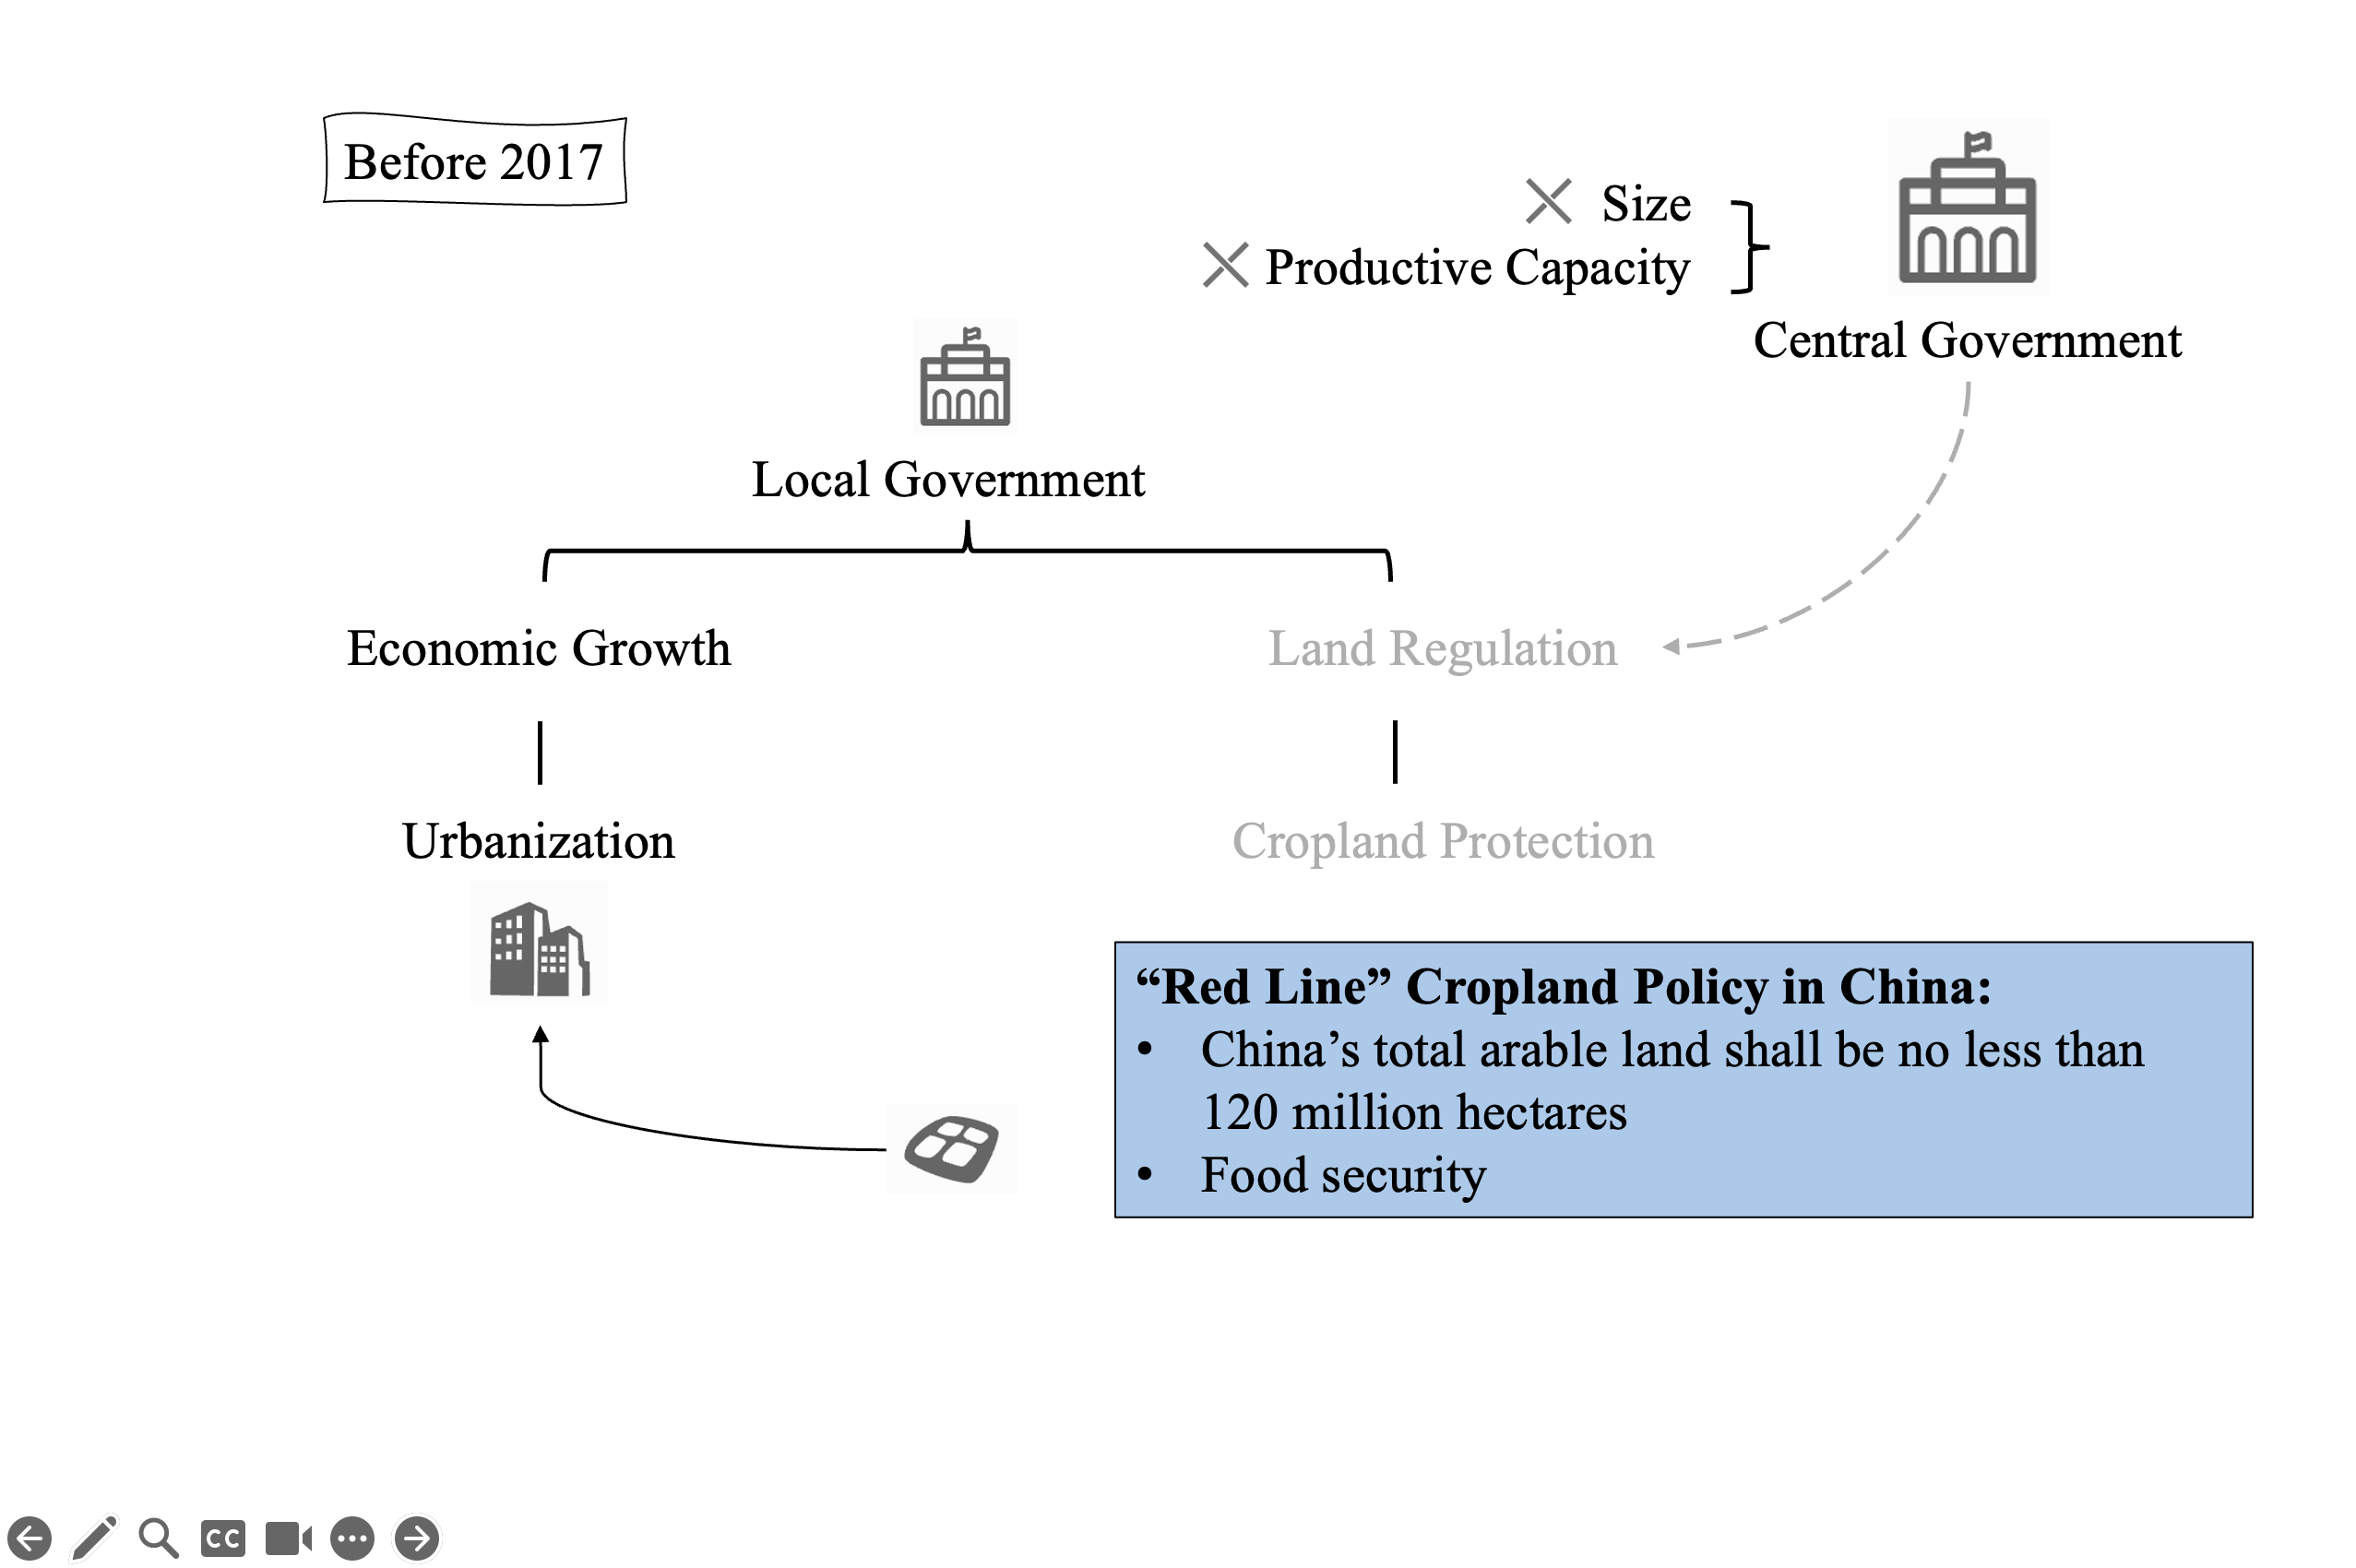
\includegraphics[width=0.9\linewidth]{frame1.png}
    \end{figure}
\end{frame}

\begin{frame}{Multitasking Bureaucrats in China: Low Multitasking Pressure}
    \begin{figure}
        \centering
        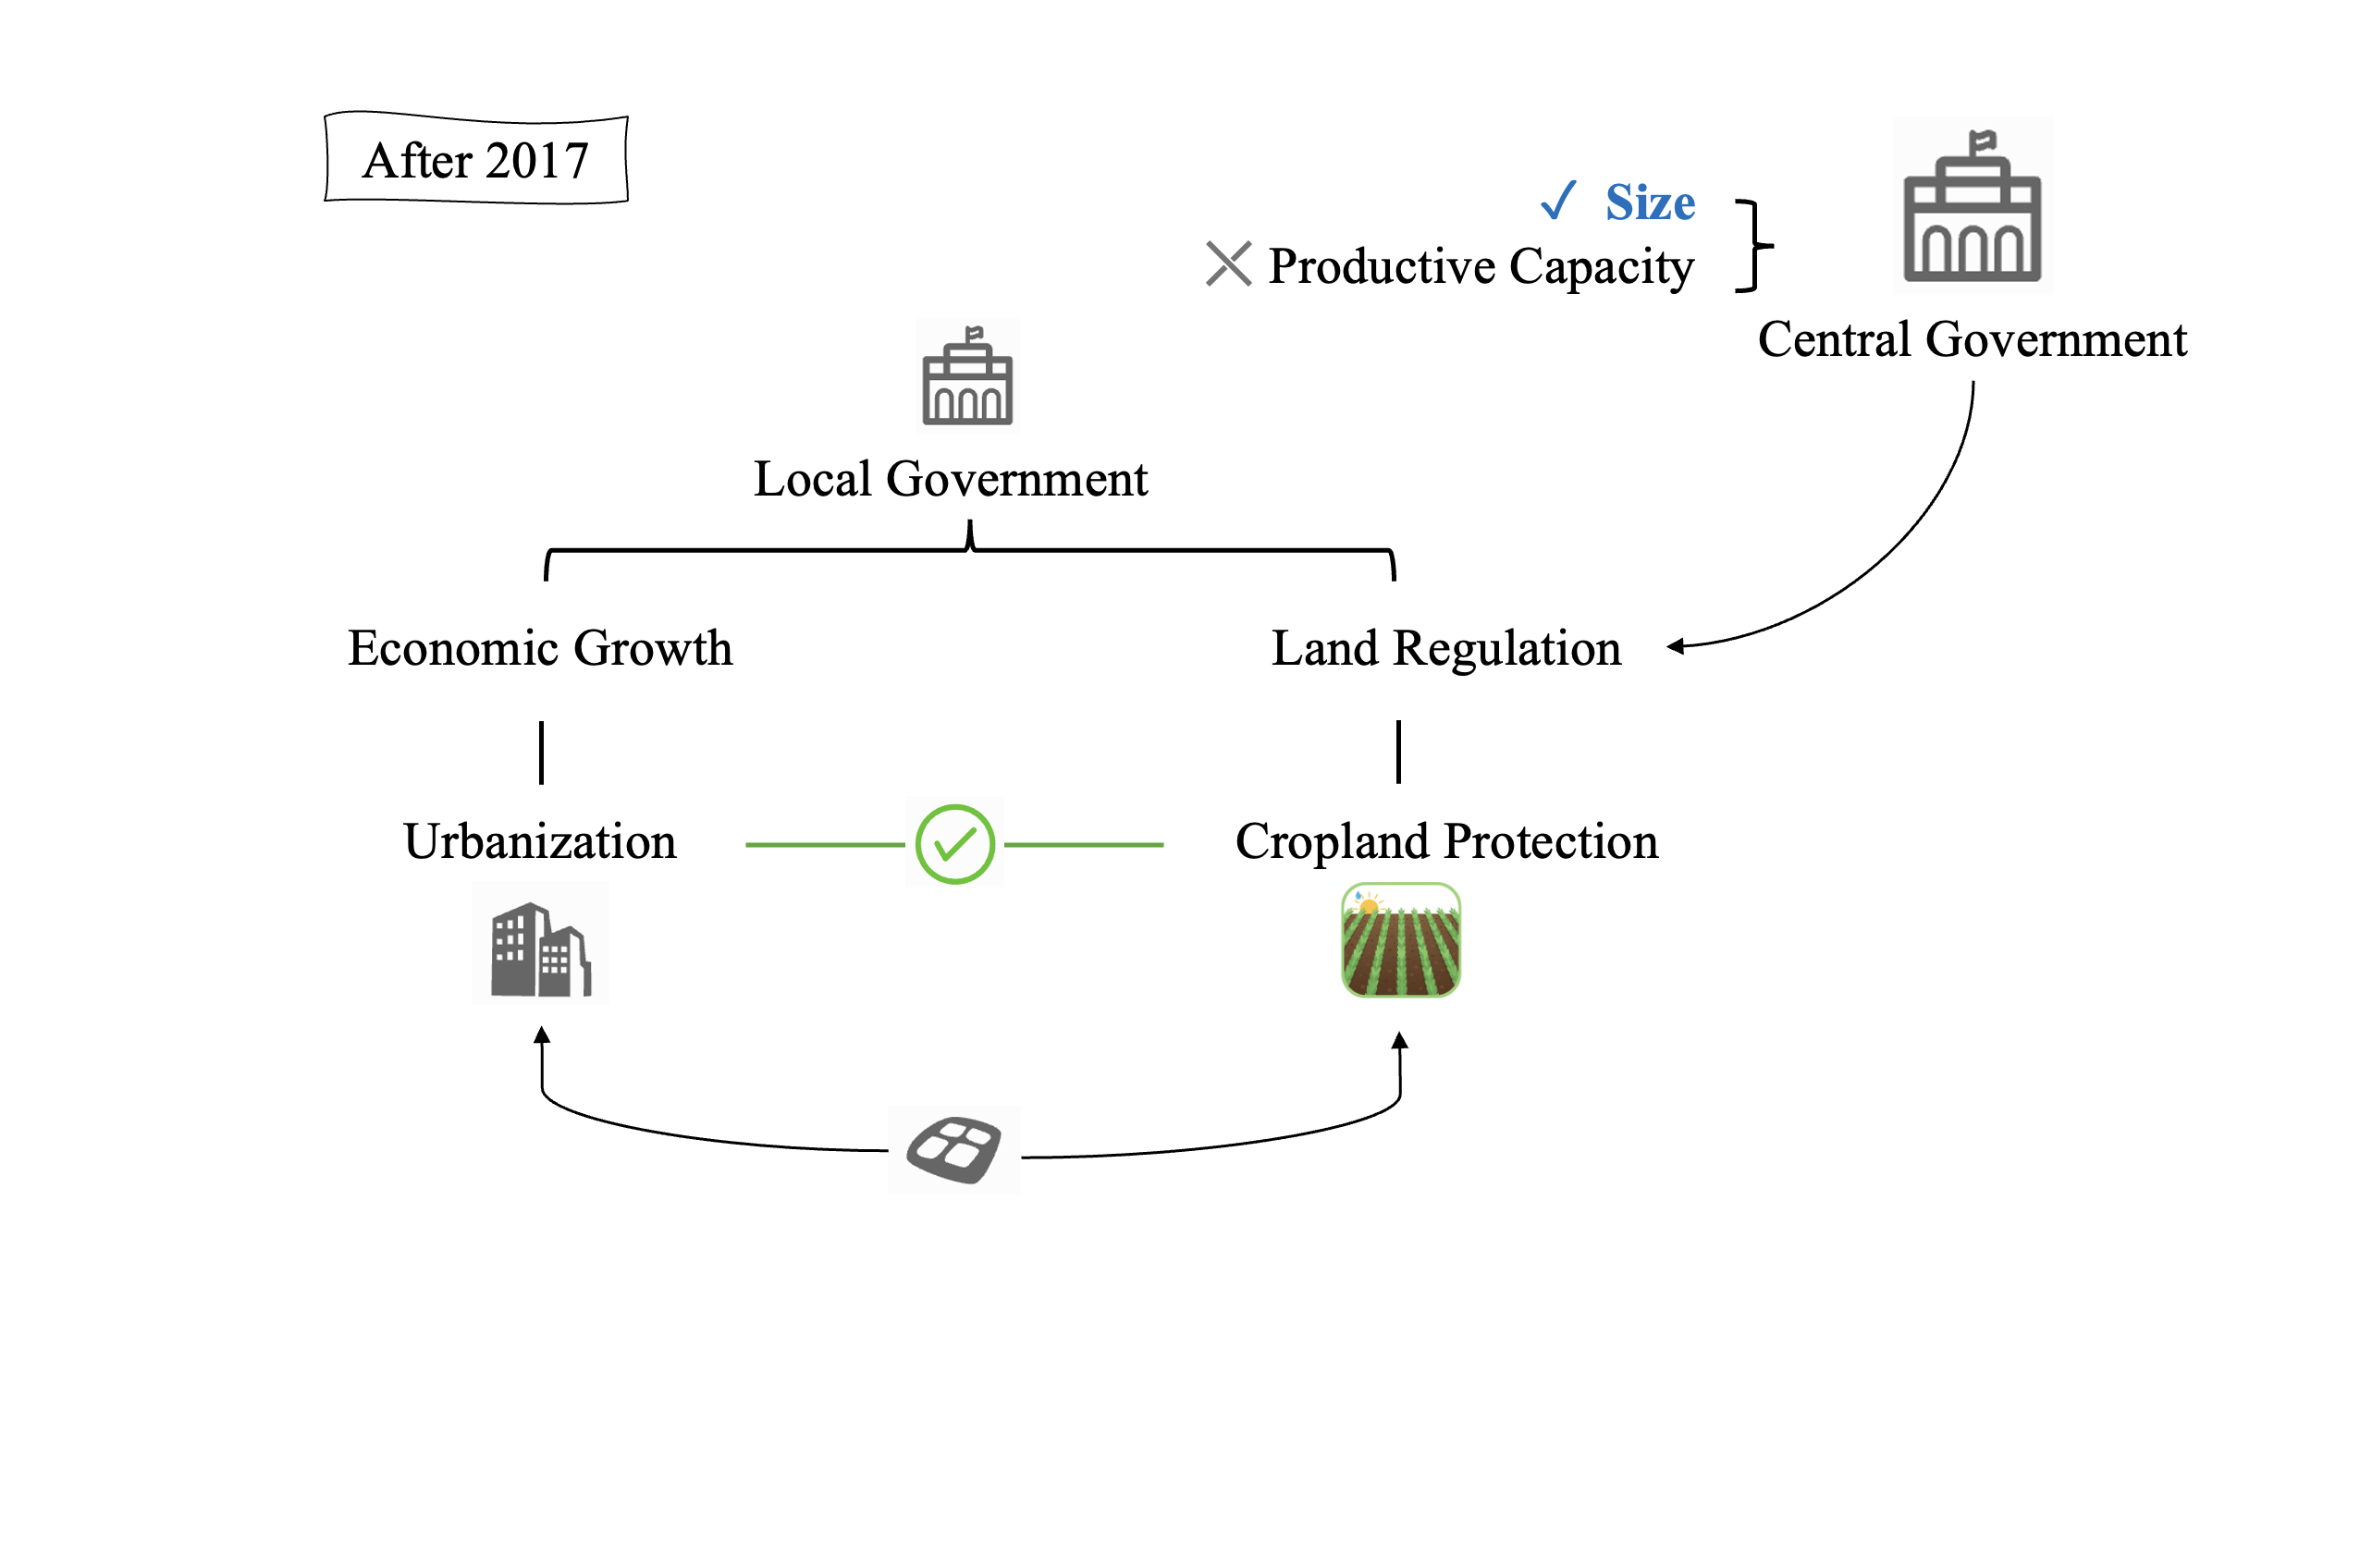
\includegraphics[width=0.9\linewidth]{frame2.png}
    \end{figure}
\end{frame}

\begin{frame}{Multitasking Bureaucrats in China: High Multitasking Pressure}
    \begin{figure}
        \centering
        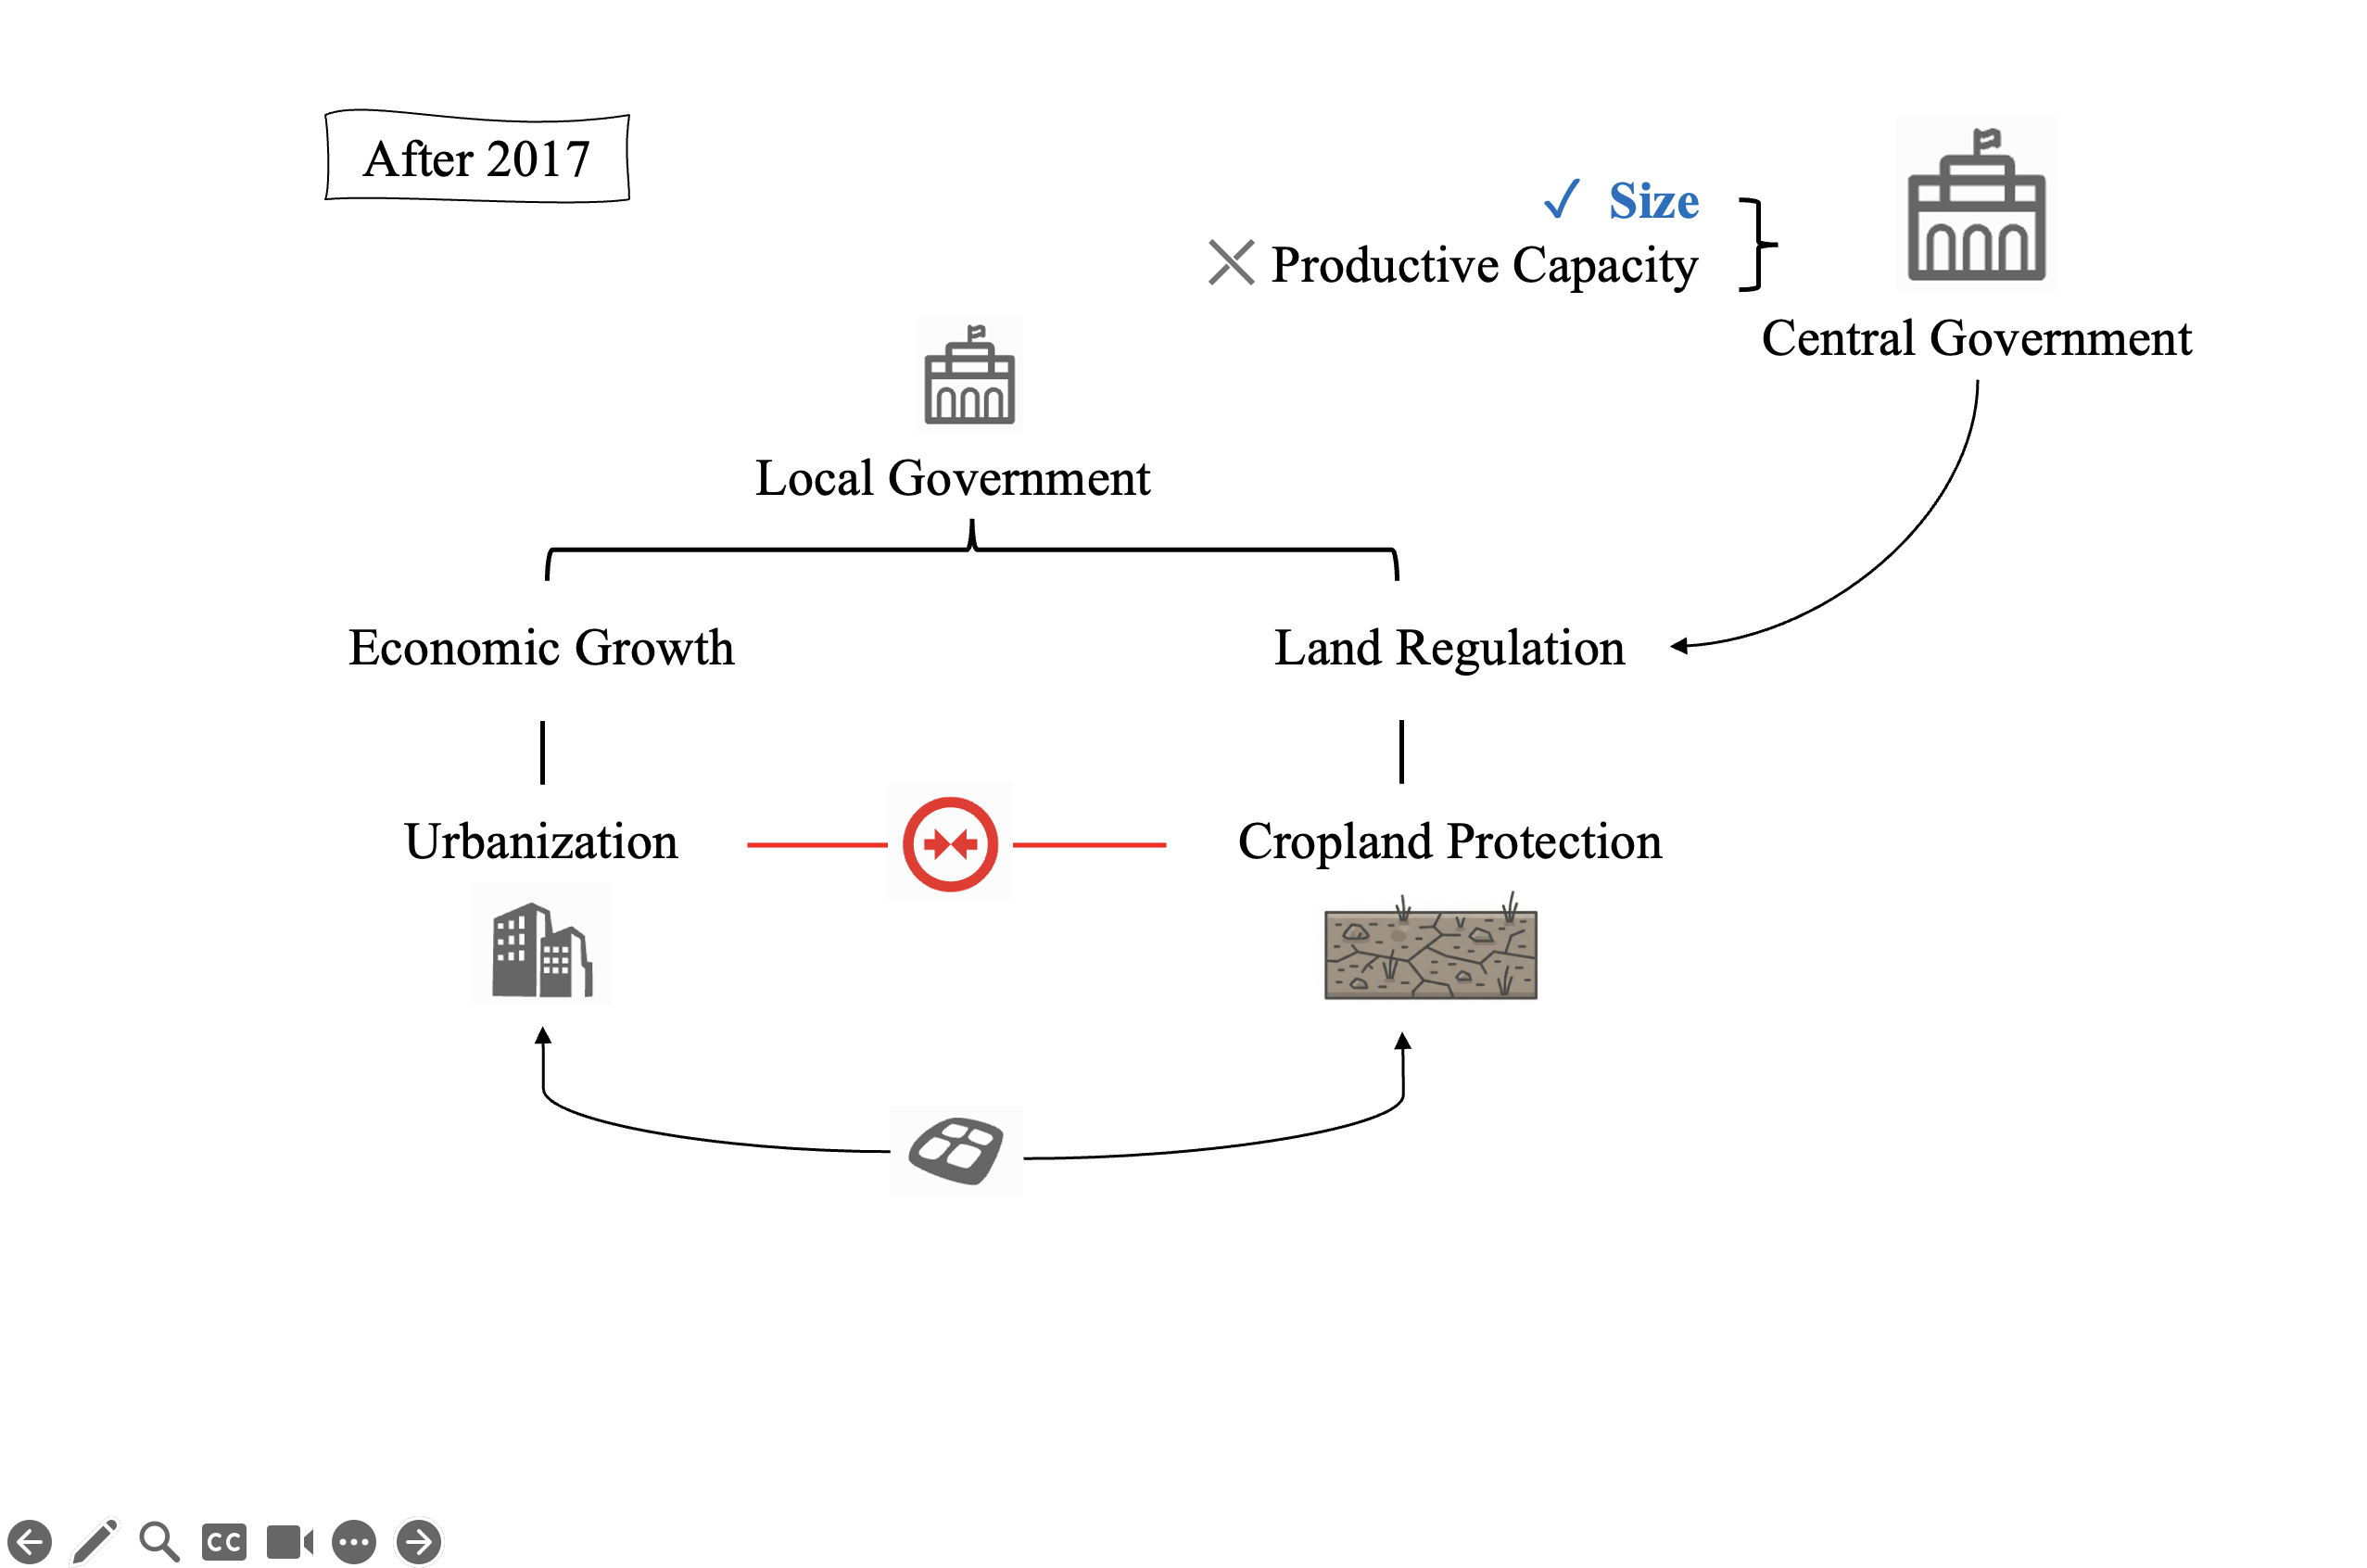
\includegraphics[width=0.9\linewidth]{frame3.png}
    \end{figure}
\end{frame}


\begin{frame}{Results Overview}
\begin{itemize}
    \item \textbf{Quantity}: In jurisdictions facing greater land protection pressure (i.e., tighter cropland replenishment targets relative to available land), land plots respond more strongly to cropland protection assessments and are more likely to be reclaimed as cropland following the policy.   
    \item \textbf{Quality}: Post-policy reclaimed cropland in high-pressure jurisdictions is more likely to be of lower soil suitability.
    \item \textbf{Efficiency}: These croplands are also more likely to be left fallow in subsequent years.
    \item \textbf{Mechanism: Multitask incentives}
    \begin{itemize}
        \item High promotion incentive + high multitask pressure (economic growth \& cropland protection) $\Rightarrow$ low-quality cropland $\uparrow$
    \end{itemize}
\end{itemize}
\end{frame}




\begin{frame}{Contribution to literature}
\begin{itemize}
    \item \textbf{Multitasking Principal–Agent Problem}
    \begin{itemize}
        \item \cite{holmstrom1991multitask}, \cite{baker1992incentive}
        \item \textbf{Applied studies in Chinese economy}: \cite{hong2025order}, \cite{fan2023land}, \cite{chen2018career}, \cite{he2020watering} $\Rightarrow$ \textcolor{blue}{trade-off between opposing tasks (economic \& environment)}
        \item \textcolor{blue}{This paper: First study on within-task distortion under imperfect monitoring: economic $\checkmark$; land protection — quantity $\checkmark$, quality $\times$ $\Rightarrow$ stricter performance measures may backfire}
    \end{itemize} 
    \item \textbf{Misallocation}
    \begin{itemize}
        \item \cite{restuccia2017land}, \cite{adamopoulos2022misallocation} $\Rightarrow$ factor allocation in agricultural production
        \item \textcolor{blue}{This paper: Land misallocation across land-use types}
    \end{itemize}
    \item \textbf{Monitoring and Information Asymmetry}
    \begin{itemize}
        \item \cite{FismanWangYe2025_StrategicCaptureOfMonitors}, \cite{axbard2024informed}, \cite{kosack2014does}
    \end{itemize}
    \item \textbf{Land Regulation}: 
    \begin{itemize}
    \item \cite{henderson2022political}, \cite{cai2017build}, \cite{hilber2016impact}, \cite{besley2000land}
    \end{itemize}
\end{itemize} 
\end{frame}


\section*{Background and Data}

\begin{frame}{Multitasking Bureaucrats and Land Regulation in China}

\begin{itemize}
    \item \textbf{Performance-based Evaluation System}: \small{\textcolor{blue}{Economic Growth} - Key Task, \textcolor{blue}{Cropland Protection} - Since 2017}
    \item \textbf{"Red Line" Cropland Policy in China}: 
\begin{itemize}
    \item 2005: The State Council released assessment measures for provincial governments\footnote{\footnotesize \href{https://www.gov.cn/gongbao/content/2005/content_129504.htm}{Document of 2005 policy}}
    \item \textcolor{blue}{2017-2018}: A revised version has been introduced to assess local land protection more \textcolor{blue}{stringently}\footnote{ \href{https://www.gov.cn/zhengce/content/2018-01/18/content_5257943.htm}{Document of 2018 policy}}
\end{itemize}
\end{itemize}

\begin{figure}[H]
    \centering
    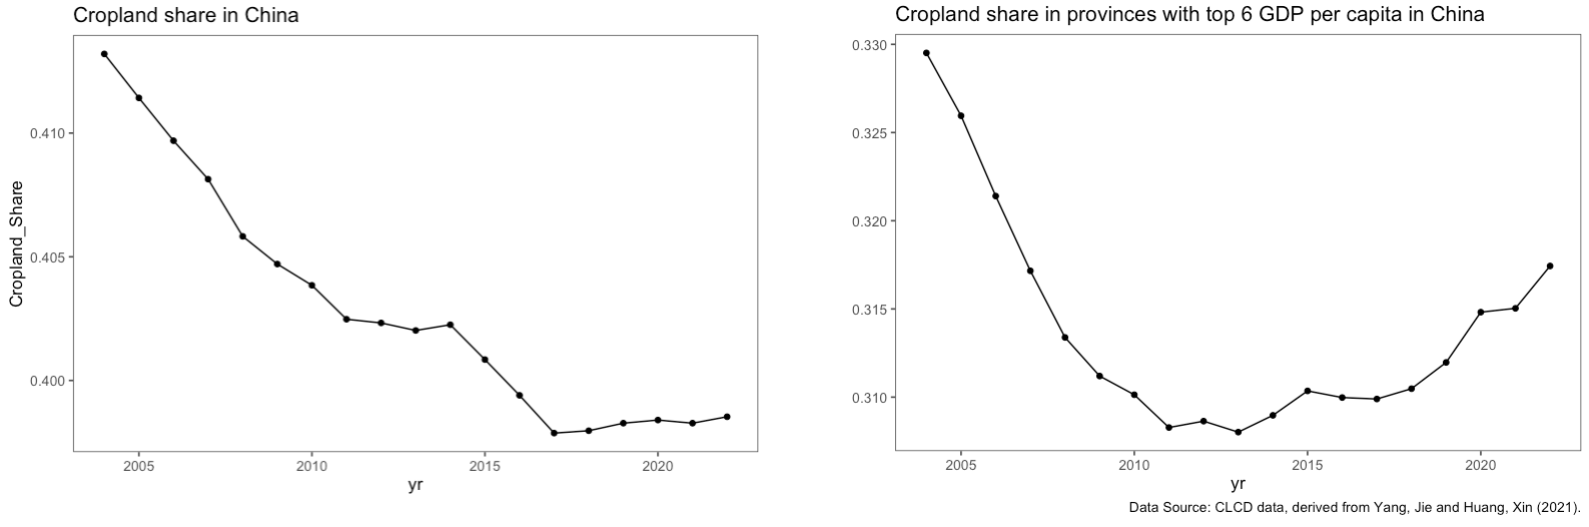
\includegraphics[width=0.8\textwidth]{cropshare_combined.png}
    \caption{Change in Cropland Share}
\end{figure}

\end{frame}

\begin{frame}{Timeline}
\begin{figure}[H]
    \centering
    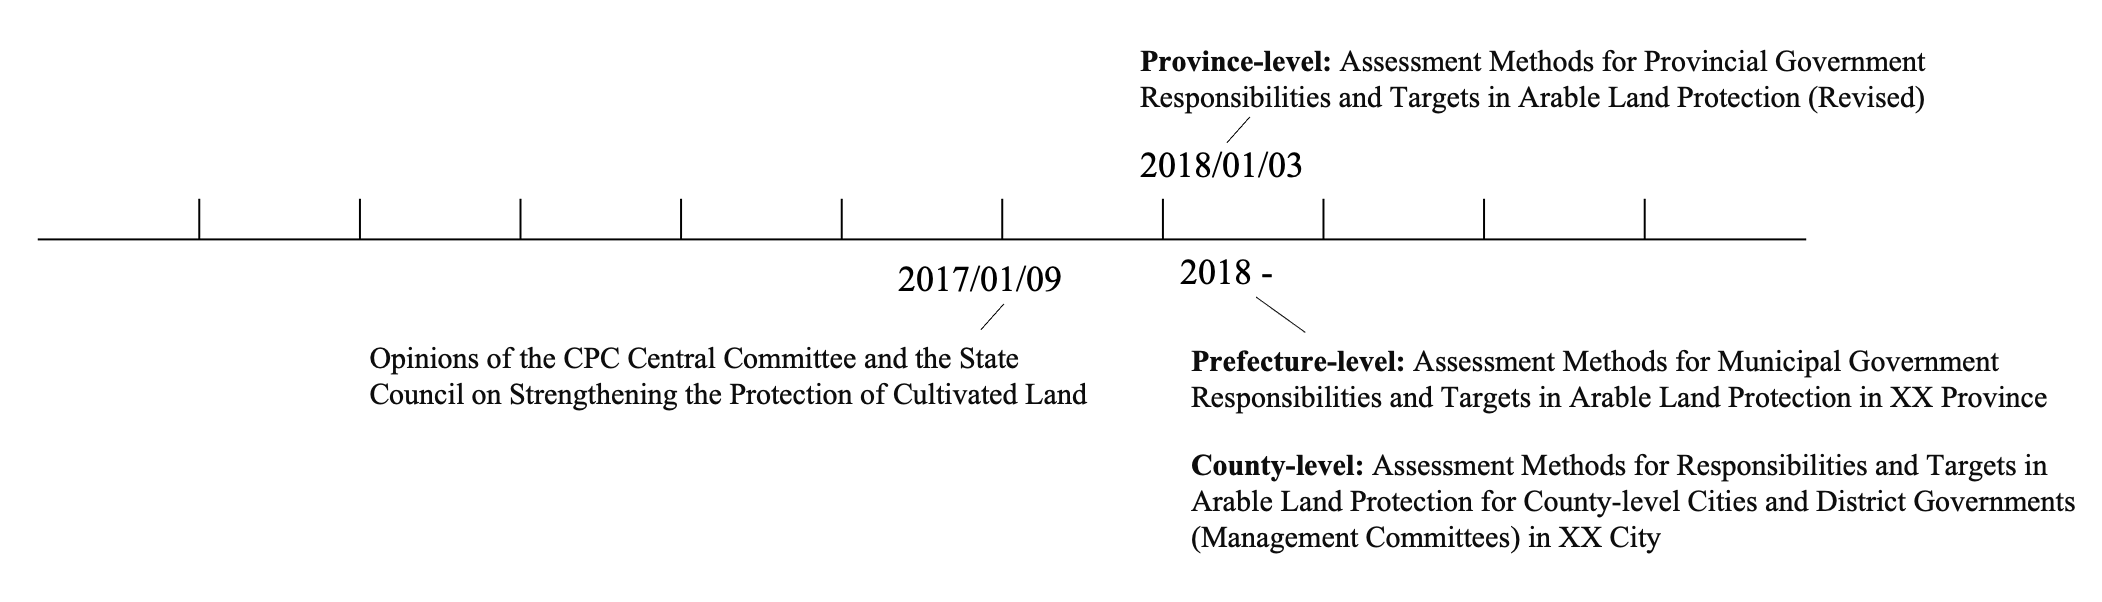
\includegraphics[width=1\textwidth]{timeline.png}
\end{figure}
\end{frame}



\begin{frame}{Background: Land Regulation and Local Implementation}
\begin{itemize}
    \item \textbf{Central government's objective}: quantity-based and productive-capacity-centered
    \item \textbf{Documented Issues}
    \begin{itemize}
        \item Implementation Distortion: $\checkmark$ quantity, X quality (People's Daily) - Maintain the \textbf{total area} of cropland rather than its quality or actual use
        \item Incentive design flaws and inadequate policy coordination (Ministry of Agriculture and Rural Affairs)
    \end{itemize}
\end{itemize}
\begin{figure}[H]
    \centering
    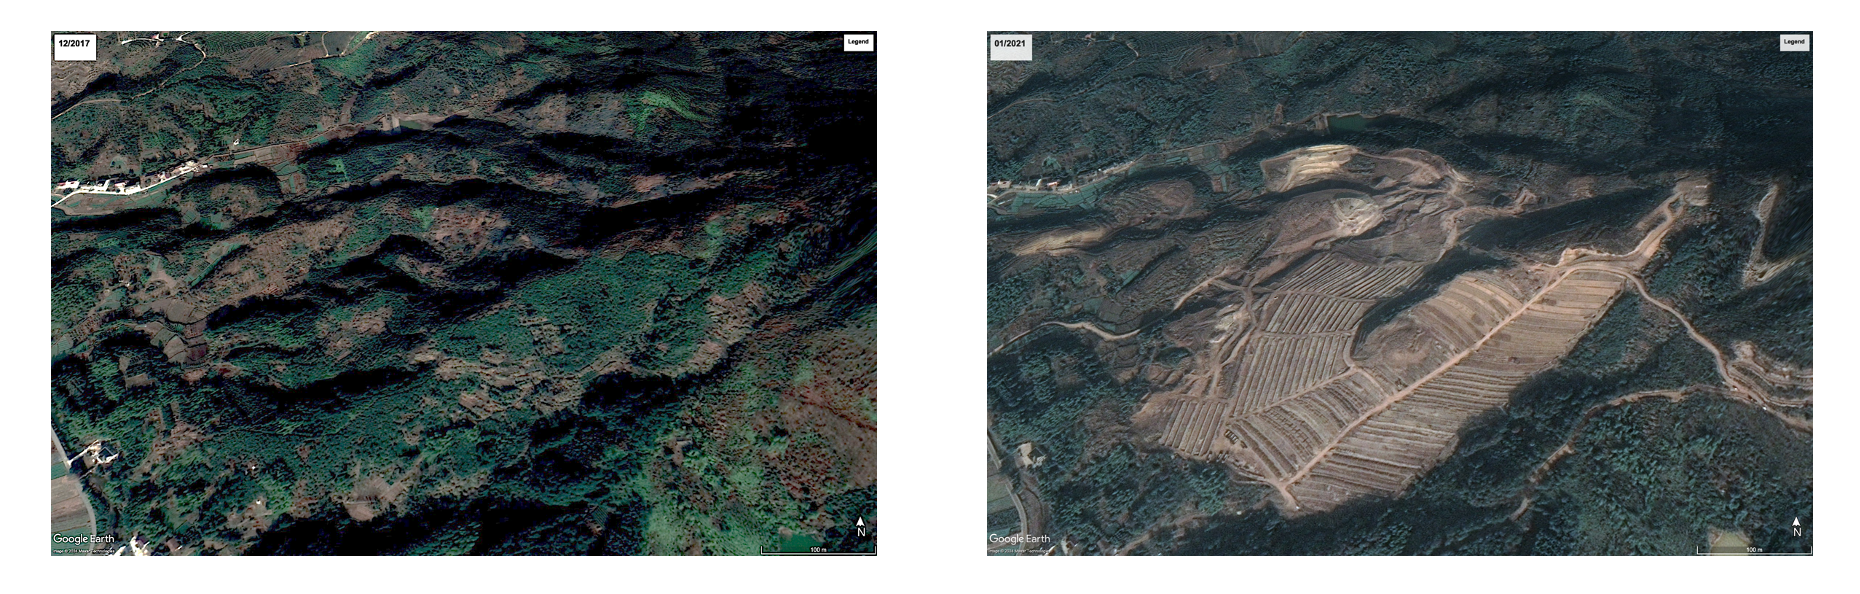
\includegraphics[width=0.9\textwidth]{anecdote_both.png}
    \caption{An example of local policy implementation: forest $\rightarrow$ terrace}
\end{figure}
\end{frame}




\begin{frame}{Data}
\begin{itemize}
    \item \textbf{Cropland Data}:
    \begin{itemize}
        \item The 30 m annual land cover dataset and its dynamics in China (2012 - 2022)
        \item Land Type: Cropland, Impervious, Water, Barren,...
    \end{itemize}
    \item \textbf{30m/15-day Fractional Vegetation Cover (FVC) dataset}: National Tibetan Plateau Data Center， derived from Landsat-based NDVI
    \item \textbf{Soil type}: The 1:1,000,000 Soil Map of China compiled by the National Soil Survey Office (1995)
    \item \textbf{Bureaucrats data}: Prefecture and province-level officials from online biographies
    \item \textbf{China county map}: Harvard Dataverse
    \item \textbf{Social-Economic data}: County Statistical Yearbook
\end{itemize}
\end{frame}

\begin{frame}{Measurement of Cropland}
\hypertarget{preliminaryresult}{}
\begin{itemize}
    \item Focus on one province - Jiangsu province: (1) High urbanization, (2) High land-use pressure
    \item 500 X 500 m grid
\begin{figure}[H]
    \centering
    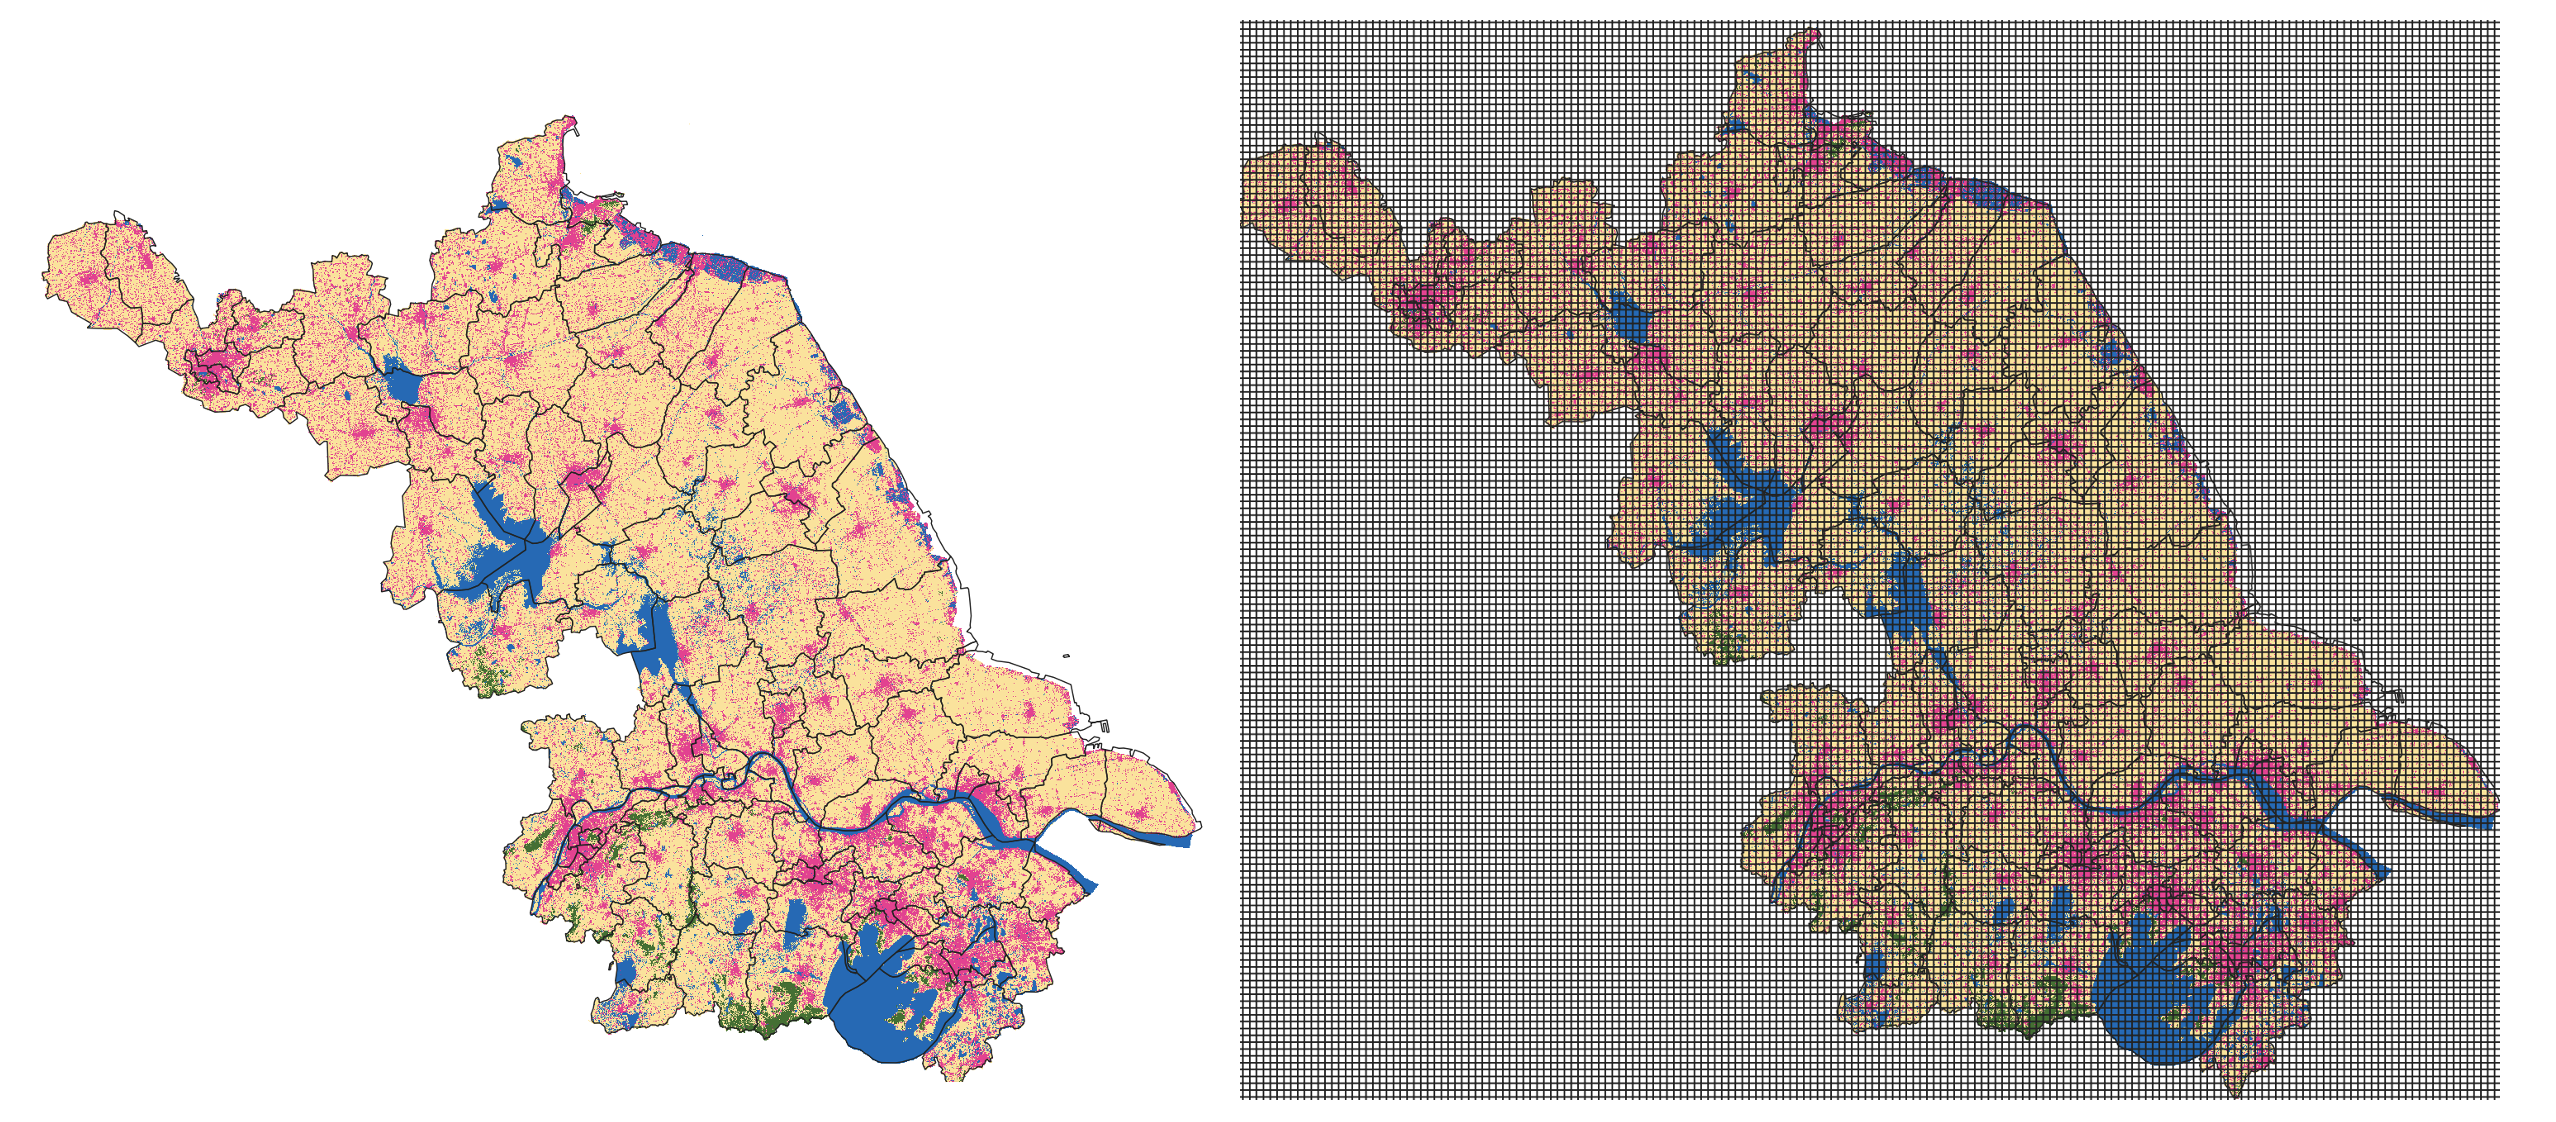
\includegraphics[width=0.7\textwidth]{jiangsu_procedure.png}
\end{figure}
\end{itemize}
\end{frame}


\begin{frame}{Measurement of Land Quality}

\textbf{Land quality is proxied by \textcolor{blue}{grid-level soil suitability}.}

\textbf{Methodological Basis}
\begin{itemize}
    \item FAO Land Evaluation Framework (FAO 1976; FAO 2007)
    \item China National Land Capability Standard (GB/T 28407--2012)
\end{itemize}

\medskip

\textbf{Mapping Soil Types to Suitability Classes}
\begin{table}[h!]
\centering
\small
\begin{tabular}{l l l}
\hline
\textbf{Score} & \textbf{FAO Class} & \textbf{Representative Soil Groups} \\
\hline
5 (S1) & Highly suitable 
& Fluvisols, Anthrosols, alluvial soils \\
4 (S2) & Moderately suitable 
& Cambisols, Luvisols, Ferralsols, Andosols \\
3 (S3) & Marginally suitable 
& Regosols, Leptosols, Cambic soils, hardpan soils \\
2 (N1) & Currently unsuitable 
& Saline soils, sodic soils, waterlogged paddy soils \\
1 (N2) & Permanently unsuitable 
& Urban land, marsh soils, water bodies, sandbars \\
\hline
\end{tabular}
\end{table}

\medskip

The score for each 500\,m $\times$ 500\,m grid cell is computed as the average of mapped soil types.

\textbf{Classification Rule:}  
Average score $\geq 3$: suitable land;  
Average score $< 3$: saline--alkaline or otherwise non-arable land.

\end{frame}

\begin{frame}{Measurement of Efficiency}

\begin{itemize}

    \item \textbf{Observation unit:} 500\,m $\times$ 500\,m grid cell

    \vspace{0.9em}
    \item \textbf{Reclaimed Cropland (Data: CLCD, 2012–2022)}
    \begin{itemize}
        \item \textbf{Cropland share:} fraction of pixels classified as cropland.
        \item \textbf{Definition:} A grid is classified as \textit{newly reclaimed} in year $t$ if its cropland share increases from below 0.6 in $t-1$ to above 0.7 in both $t$ and $t+1$ (0.7 is the pre-policy mean).
    \end{itemize}

    \vspace{0.9em}
    \item \textbf{Efficiency Measure (Data: FVC, 2010–2022)}
    \begin{itemize}
        \item FVC ranges from 0–100 (scaled by 0.01); higher values indicate denser vegetation cover.
    \end{itemize}

    \vspace{0.9em}
    \item \textbf{Definition of Fallow Rate}
    \begin{itemize}
        \item For each newly reclaimed grid $i$, the \textbf{fallow rate} is defined as the share of post-reclamation years in which annual average FVC falls below 0.20 (bottom 25\% of the distribution).
    \end{itemize}

\end{itemize}

\end{frame}

\begin{frame}{Measurement of Land Protection Pressure}

\textbf{Policy Background}

\begin{itemize}\setlength{\itemsep}{8pt}

\item[(1)] \textbf{Cropland Occupation–Replenishment Rule.}  \\
Under the national “cropland occupation–supplement balance’’ policy, a county that converts cropland to construction land must replenish an \textit{equal amount} of cropland elsewhere.

\item[(2)] \textbf{Replenishment is not necessarily local.}  
Local governments may fulfill their replenishment obligations outside their own jurisdiction:
\begin{itemize}
    \item within the same county,
    \item \textcolor{blue}{if insufficient, within the same prefecture (across counties)\footnotemark[1]}, 
    \item if still insufficient, in other counties within the same province with similar resource conditions\footnotemark[1].
\end{itemize}

\textcolor{blue}{This creates a \textit{capacity constraint} determined by the non-core (non-urban) area within a prefecture.}  

\end{itemize}

% ---- shared footnote text ----
\footnotetext[1]{Jurisdictions that cannot meet the balance requirement can purchase supplementary cropland indicators through a paid, auction-based transaction platform.}

\end{frame}




\begin{frame}{Measuring County-Level Land-Pressure Exposure}

\bigskip

\textbf{Definition: Land-Pressure Exposure}

\begin{equation}*
\text{Pressure}_{c}
=
\left(
\frac{\text{Obligation}_{p}}
     {\text{TotalLand}_{p}}
\right)
\times 
\text{LandShare}_{c},
\end{equation}*

\begin{itemize}
    \item $\text{Obligation}_{p}$: Total cropland-replenishment obligation assigned to the \emph{core urban districts}\footnote{Specified in Land Use Master Plan. Fully core = 1, partly core 0.5, non-core = 0.} of prefecture $p$ under the provincial planning targets (set in 2017, effective 2018--2020).  
    \item $\text{TotalLand}_{p}$: Total area of \emph{available land}\footnote{1 - impervious - water} in prefecture $p$ outside the urban districts. This is the prefecture’s ``land reservoir’’ available for real cropland replenishment.
    \item $\text{LandShare}_{c}$: County $c$'s share of this reservoir:
    \[
    \text{LandShare}_{c}
    =
    \frac{\text{AvailableLand}_{c}}
         {\sum_{c' \in p}\text{AvailableLand}_{c'}}.
    \]
\end{itemize}

\bigskip

\end{frame}






\begin{frame}{Motivating Fact}
    \begin{figure}
        \centering
        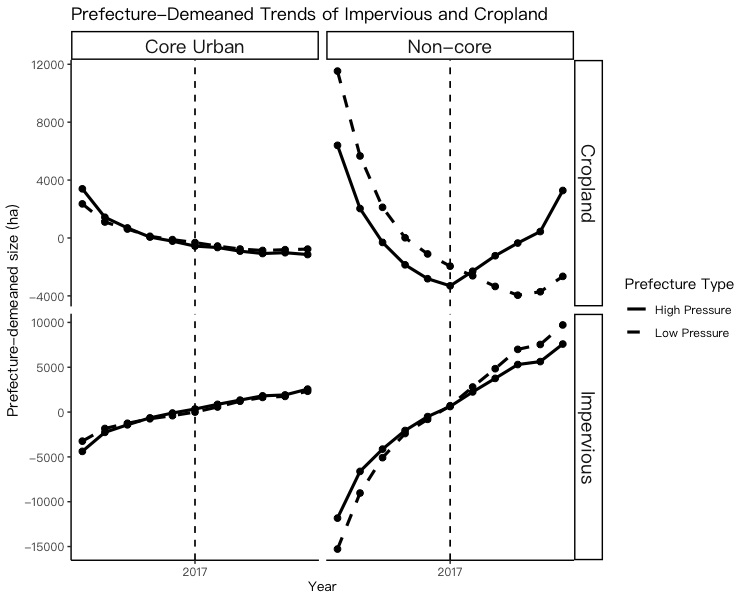
\includegraphics[width=0.58\linewidth]{Motivating_size.png}
        \label{fig:placeholder}
    \end{figure}
\end{frame}

\begin{frame}{Motivating Fact}
    \begin{figure}
        \centering
        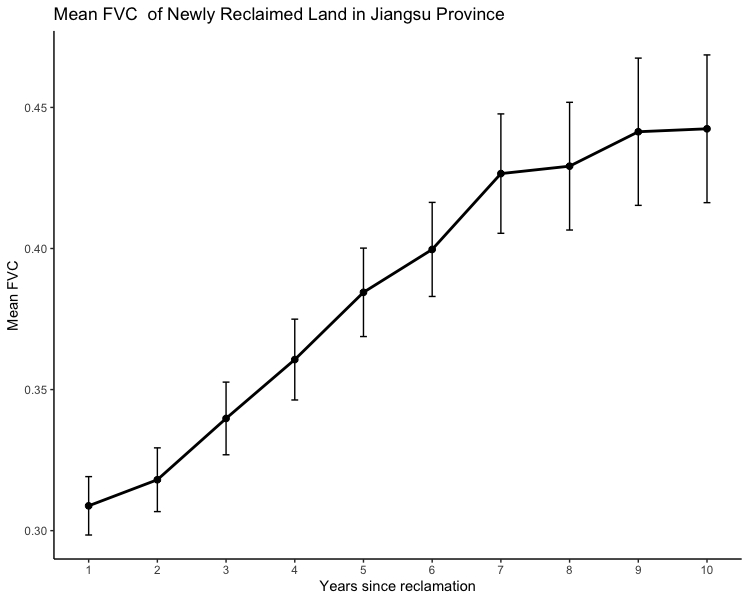
\includegraphics[width=0.58\linewidth]{Motivating_fvc.png}
        \label{fig:placeholder}
    \end{figure}
\end{frame}

\begin{frame}{Motivating Fact}
    \begin{figure}
        \centering
        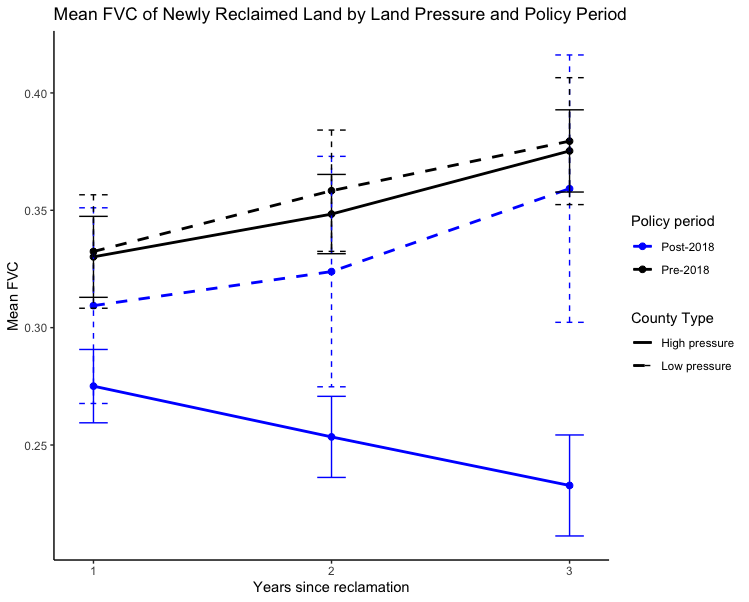
\includegraphics[width=0.58\linewidth]{Motivating_reclaimed_group.png}
        \label{fig:placeholder}
    \end{figure}
\end{frame}

\section*{Conceptual Framework}

\begin{frame}{Plot Types}

\textbf{Plot-level characteristics.}  
Each plot $j$ has two fundamental attributes:

\begin{itemize}
  \item \textbf{Economic potential} $p_j$:  
        \begin{itemize}
            \item reflects the economic value of converting the plot to construction land,
            \item determined by access to infrastructure, proximity to urban centers, and other locational advantages.
        \end{itemize}

  \item \textbf{Land quality} $q_j$:  
        intrinsic agronomic conditions (soil suitability, slope/ruggedness, water availability).
\end{itemize}

\medskip

\textbf{Production function.}
\[
y_j = f(q_j, e_j),
\]
where $e_j$ is cultivation effort (irrigation, planting, early maintenance).

\medskip

\textbf{Higher land quality implies:}
\begin{itemize}
    \item higher marginal returns to effort ($f_{qe}>0$), and
    \item lower cost of reaching a given productivity level.
\end{itemize}

\end{frame}

\begin{frame}{Government's Problem}

\textbf{Central government.}
\begin{itemize}
  \item Aims to preserve agricultural output through both \emph{cropland area} and \emph{cropland productivity}.
  \item In practice, monitoring is:
  \begin{itemize}
      \item $\checkmark$ \textbf{Area}: fully observable,
      \item $\boldsymbol{\times}$ \textbf{Quality / Productivity}: not directly observable.
  \end{itemize}
\end{itemize}

\medskip

\textbf{Local government incentives.}
\begin{itemize}
  \item Objectives: (i) meet economic growth targets, and  
        (ii) fulfill cropland-area mandates at minimal fiscal and political cost.
  \item \textbf{Local governments do not internalize the agricultural outcome $y_j$.}
\end{itemize}

\end{frame}

\begin{frame}{Land Pressure, Local Trade-offs, and Fallowing Mechanism}

\textbf{Land-pressure heterogeneity.}
\begin{itemize}
  \item Low-pressure cities possess substantial low-$p_i$, high-$q_i$ land reserves.
  \item High-pressure cities lack such land and face a trade-off:
  \begin{enumerate}
     \item reclaim low-$q_i$ land at low fiscal cost; or
     \item obtain high-$q_i$ cropland at high cost 
           (quota trading).
  \end{enumerate}
  \item Because option (2) is substantially more expensive,  
        high-pressure cities choose option (1)  
        $\Rightarrow$ \textcolor{blue}{lower cropland quality after 2017}.
\end{itemize}

\medskip

\textbf{Farmers’ response and fallowing.}
\begin{itemize}
  \item Farmers and firms care about $y_j = f(q_j,e_j)$, not the administrative area target.
  \item On low-quality land, the return to effort is low $\Rightarrow$ weak cultivation incentives.
  \item Result: newly reclaimed cropland in high-pressure cities is more likely to remain fallow  
        $\Rightarrow$ \textcolor{blue}{lower FVC and poor vegetation recovery after 2017}.
\end{itemize}

\end{frame}

\section{Identification Strategy}

\begin{frame}{Identification and Empirical Specification}

\begin{block}{Event-Study Specification (TWFE):}
\[
    \text{crop\_share}_{i c t}
    =
    \sum_{k \neq -1}
    \beta_k
    \Big(
        \text{Pressure}_{c} 
        \times 
        \text{Event}_{k,t}
    \Big)
    +
    \mu_i
    +
    \lambda_t
    +
    \varepsilon_{i c t}.
\]
\end{block}

\bigskip

\textbf{Notation.}
\begin{itemize}\setlength{\itemsep}{6pt}
    \item $i$: grid cell;  $c$: county; $t$: year.
    \item $\text{Pressure}_{c}$: county-level land protection pressure
    \item $\text{Event}_{k,t}$: indicator for event time $k$ relative to 2017  
    \item $\mu_i$: grid fixed effects.
    \item $\lambda_t$: year fixed effects。
\end{itemize}



\end{frame}




\begin{frame}{Empirical Strategy for Reclaimed Land: Cohort DID}

\begin{itemize}

    \item \textbf{Observation unit:} Newly reclaimed grid cell $i$
    \begin{itemize}
        \item Reclamation cohort: $t_0(i) \in \{2013,\ldots,2021\}$
        \item Post-reclamation years: $s$
        \item Outcome: $Y_{i,s}=1$ if grid $i$ is fallow in $t_0(i)+s$
    \end{itemize}

    \vspace{0.8em}

    \item \textbf{Treatment intensity:}
    \[
        W_i = 1\{t_0(i)\ge 2018\} \times \text{Pressure}_{c(i)}
    \]

    \vspace{0.6em}

    \item \textbf{Cohort-DID specification:}
    \[
        Y_{i,s}
        =
        \alpha_{c(i)} 
        + 
        \mu_{t_0(i)}
        +
        \delta_s
        +
        \beta W_i
        +
        X_i'\gamma
        +
        \varepsilon_{i,s}.
    \]

\end{itemize}

\bigskip

\textbf{Notation.}
\begin{itemize}\setlength{\itemsep}{6pt}
    \item $c(i)$: county of grid $i$.
    \item $\alpha_{c(i)}$: county fixed effects.
    \item $\mu_{t_0(i)}$: cohort (reclamation year) fixed effects.
    \item $\delta_s$: years-since-reclamation fixed effects.
    \item $\text{Pressure}_{c(i)}$: county-level land protection pressure.
\end{itemize}

\end{frame}





\section*{Empirical Results}

\begin{frame}{Cropland Expansion}

\begin{figure}[H]
    \centering
    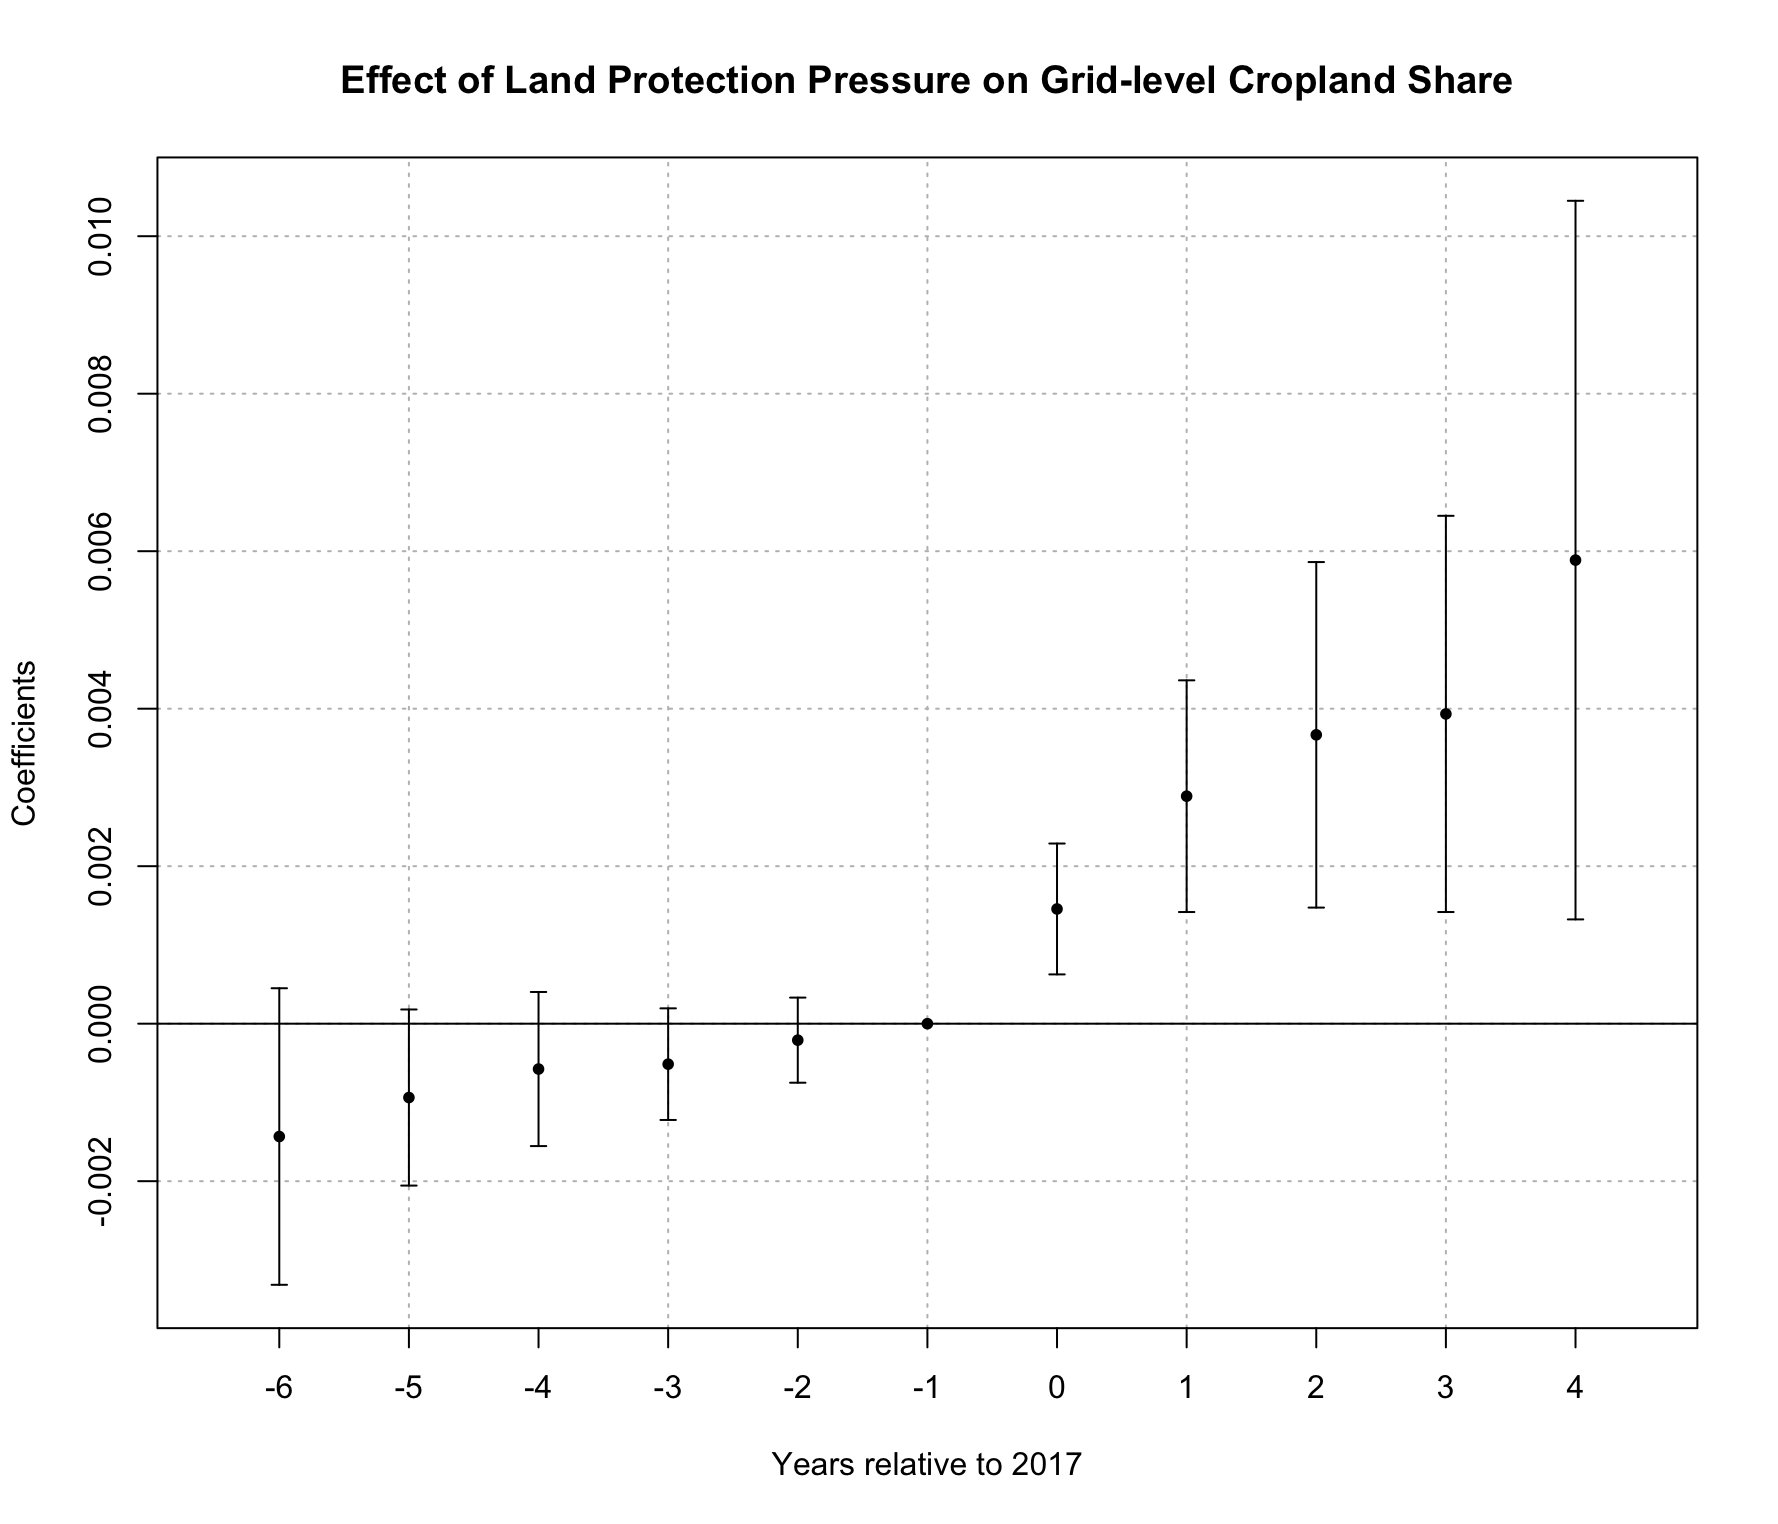
\includegraphics[width=0.6\textwidth]{res_size.png}
\end{figure}
\end{frame}

\begin{frame}{Soil Quality}
     \begin{table}[htbp]\centering
        
\begin{tabular}{lcccc}
\toprule
& \multicolumn{2}{c}{Soil Suitability (1–5)} 
& \multicolumn{2}{c}{Soil Suitability($\geq 3$)} \\
\cmidrule(lr){2-3} \cmidrule(lr){4-5}
& (1) & (2) & (3) & (4) \\
\midrule

Land Protection Pressure × Post 
& -0.183\textsuperscript{***} 
& -0.202\textsuperscript{***} 
& -0.051\textsuperscript{***}  
& -0.051\textsuperscript{***} \\
& (0.058) & (0.064) & (0.018) & (0.017) \\[2pt]

Control Mean
& 3.45 & 3.45 & 0.596 & 0.596 \\

County Controls X Year
&  & $\checkmark$ &  & $\checkmark$ \\

County \& Cohort FE 
& $\checkmark$ & $\checkmark$ & $\checkmark$ & $\checkmark$ \\

Number of Counties
& 52 & 52 & 52 & 52 \\

Num. Obs. 
& 939 & 939 & 939 & 939 \\

R$^{2}$ 
& 0.414 & 0.417 & 0.422 & 0.426 \\

\bottomrule
\end{tabular}




    \end{table}
\end{frame}

\begin{frame}{Efficiency}
    \begin{table}[htbp]\centering
        
\begin{tabular}{lcc}
\toprule
& \multicolumn{2}{c}{Fallow} \\
\cmidrule(lr){2-3}
& (1) & (2) \\
\midrule

Land Protection Pressure × Post 
    & 0.055\textsuperscript{***} 
    & 0.055\textsuperscript{***} \\
& (0.015) & (0.017) \\[2pt]

Control Mean & 0.26 & 0.26 \\

County Controls X Year
    &  
    & $\checkmark$ \\

County \& Cohort FE 
    & $\checkmark$ 
    & $\checkmark$ \\

Year since Reclamation FE
    & $\checkmark$
    & $\checkmark$ \\

Number of Counties
    & 54 & 54 \\

Num. Obs.
    & 3243 & 3221 \\

R$^{2}$
    & 0.230 & 0.229 \\
\bottomrule
\end{tabular}

{\footnotesize
\textit{Notes}: Standard errors in parentheses.
$^{*} p<0.1$, $^{**} p<0.05$, $^{***} p<0.01$.
\par}

    \end{table}
\end{frame}

\begin{frame}{Efficiency}
   \begin{figure}
        \centering   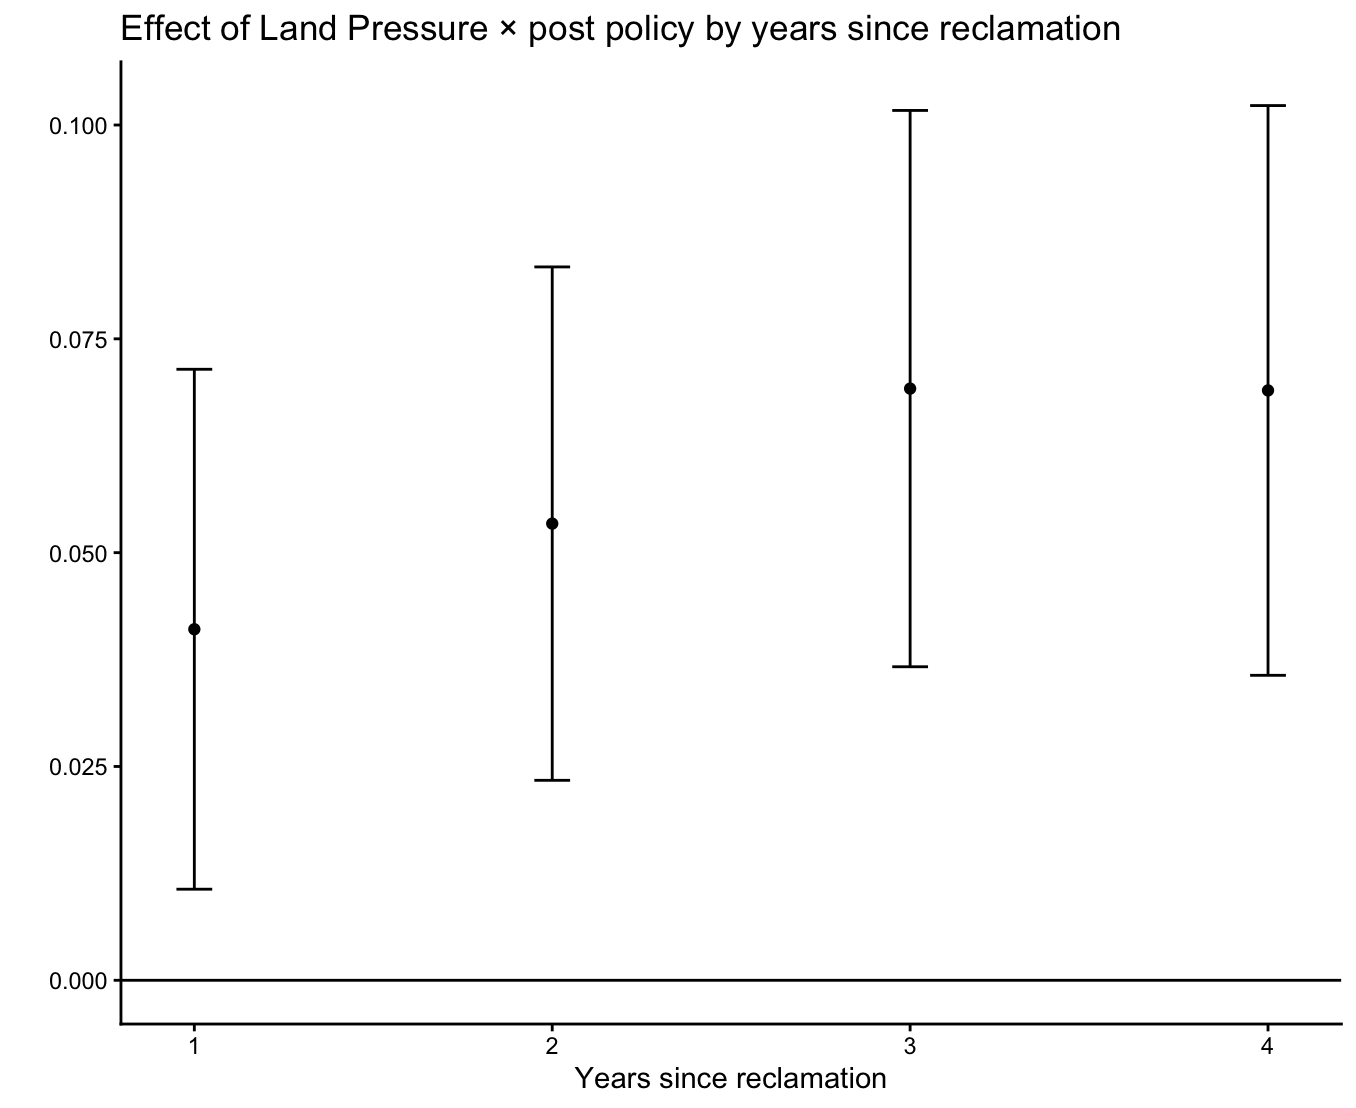
\includegraphics[width=0.59\linewidth]{res_fallow_s.png}
    \end{figure}
\end{frame}

\begin{frame}{Efficiency}
   \begin{figure}
        \centering   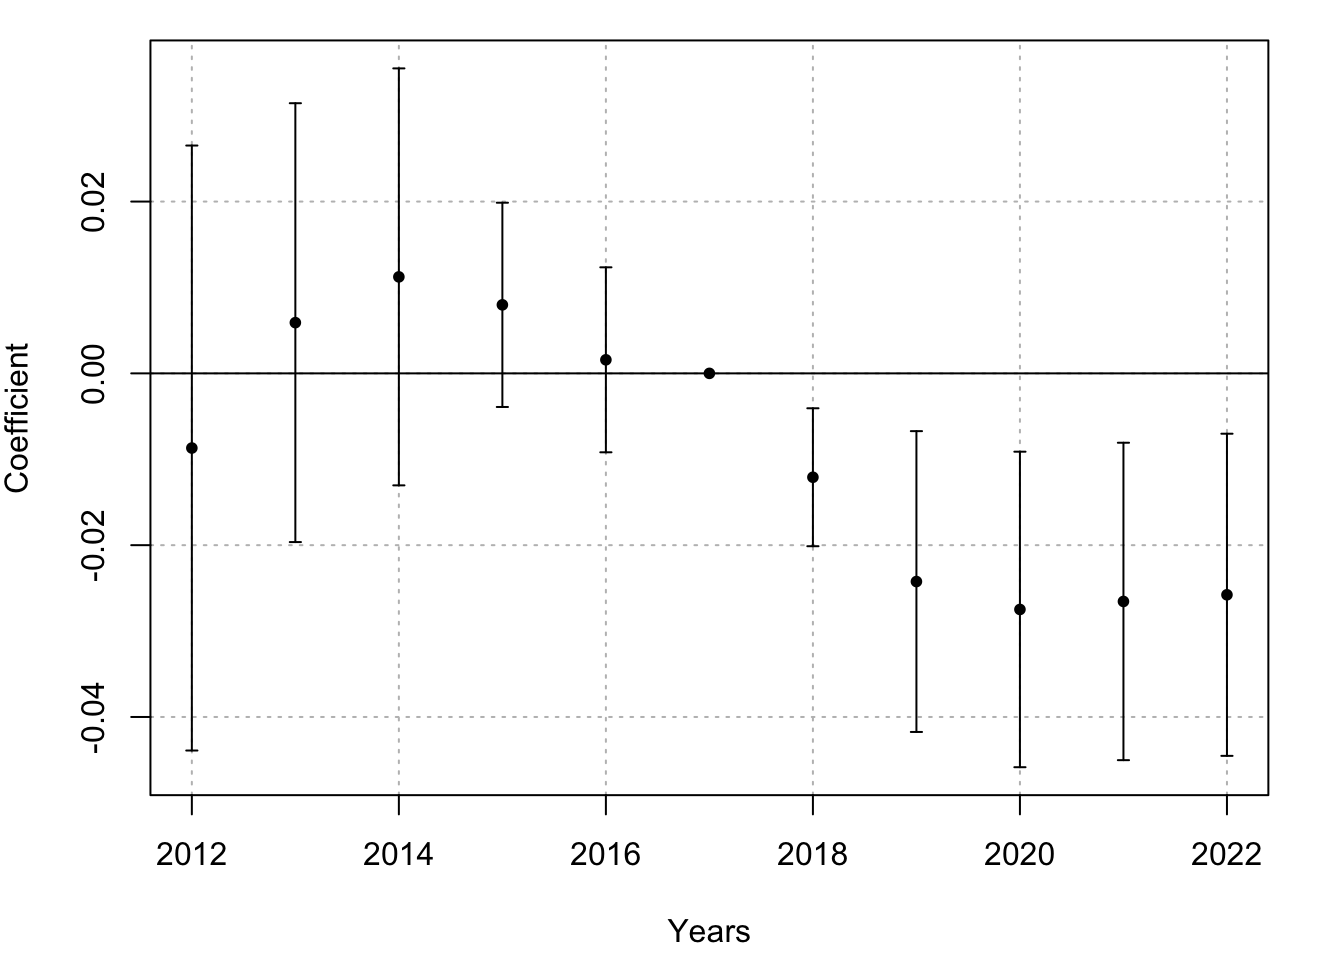
\includegraphics[width=0.59\linewidth]{res_fvc_event.png}
    \end{figure}
\end{frame}


\section*{Mechanism}

\begin{frame}{Mechanism: Multi-task Incentives and Land Quality}

\begin{itemize}

    \item \textbf{Hypothesis:}  
    Binding multi-task incentives  
    $\Rightarrow$ incentive to meet land targets at minimal cost  
    $\Rightarrow$ reclamation on low-quality land  
    $\Rightarrow$ low cultivation and high fallowing.

    \item Binding \textcolor{blue}{multi-task incentives are strongest} when:
    \begin{itemize}
        \item \textcolor{blue}{Promotion window: Age $< 58$}
        \item \textcolor{blue}{High multi-task pressure: reclamation year $< 2020$ (pre-COVID \& before the land inspection)}
    \end{itemize}

\end{itemize}

\begin{table}[htbp]\centering
\scalebox{0.85}{
\begin{tabular}{lcc}
\toprule
& (1) Soil Suitability (1--5) 
& (2) Soil Suitability ($\geq 3$) \\
\midrule

Pressure $\times$ Post 
& $-0.168$\textsuperscript{***} 
& $-0.046$\textsuperscript{***} \\
& $(0.051)$ & $(0.016)$ \\[0.4em]

Strong Incentive $\times$ Pressure $\times$ Post 
& $-0.089$\textsuperscript{**} 
& $-0.029$\textsuperscript{*} \\
& $(0.043)$ & $(0.014)$ \\[0.4em]

County \& Cohort FE 
& $\checkmark$ & $\checkmark$ \\
Num. Counties 
& 52 & 52 \\
Num. Obs. 
& 939 & 939 \\
R$^{2}$ 
& 0.374 & 0.383 \\
\bottomrule
\end{tabular}}

\end{table}

\end{frame}

\begin{frame}{Soil Quality and Fallowing}
    \begin{table}[htbp]\centering

\scalebox{0.85}{
\begin{tabular}{lcc}
\toprule
& \multicolumn{2}{c}{Outcome: Fallow} \\
\midrule
& (1) Soil Quality (1--5) 
& (2) Soil Quality ($\geq 3$) \\
\midrule

Pressure $\times$ Post 
& $0.099^{***}$ 
& $0.084^{***}$ \\
& $(0.030)$ & $(0.025)$ \\[0.4em]

Soil Suitability $\times$ Pressure $\times$ Post 
& $-0.010^{**}$ 
& $-0.034^{*}$ \\
& $(0.005)$ & $(0.018)$ \\[0.4em]

County, Cohort \& Year FE 
& $\checkmark$ & $\checkmark$ \\
Num. Counties 
& 52 & 52 \\
Num. Obs. 
& 3,185 & 3,185 \\
R$^{2}$
& 0.229 & 0.229 \\
\bottomrule
\end{tabular}}




\end{table}
\end{frame}


\section*{Robustness Check}

\begin{frame}{Robustness Check}
\begin{itemize}
    \item Alternative Definitions of Land Pressure
    \begin{itemize}
    
        \item \textit{Obligation\_p}: Reclassification of \textbf{core-urban districts}  
        \begin{itemize}
            \item Original: fully core = 1, \textcolor{blue}{partly core = 0.5}, non-core = 0  
            \item Robustness: fully core = 1; \textcolor{blue}{partly core and non-core = 0}
        \end{itemize}

        \item \textit{TotalLand\_p}: Definition of \textbf{available land}  
        \begin{itemize}
            \item Original: \textcolor{blue}{excludes water and impervious area}
            \item Robustness: \textcolor{blue}{includes all land types}
        \end{itemize}
        \end{itemize}
    \item Sensitivity to Reclaimed-Land Classification
    \begin{itemize}
        \item Baseline: 
        $\text{Reclaimed}_t = 1$ if 
        $\{CropShare_{t-1} < 0.60\} \;\land\; 
        \{CropShare_t, CropShare_{t+1} > 0.70\}$, 
        where $0.70$ is the pre-treatment mean.
        \item Robustness:  
        \textcolor{blue}{$0.60 \;\rightarrow\; 0.55\text{–}0.65$ for the previous year's threshold.}
    \end{itemize}

    \item Sensitivity to Fallow Definition
    \begin{itemize}
        \item Baseline: 
        $\text{Fallow}=1$ if $\text{FVC} < 0.20$, 
        where $0.20$ corresponds to the bottom $25\%$.
        \item Robustness: 
        \textcolor{blue}{$0.20 \;\rightarrow\; 0.13\text{–}0.20$.}
     \end{itemize}
\end{itemize}
\end{frame}




\section*{Conclusion}
\begin{frame}{Next Steps}
\begin{itemize}
    \item \textbf{Empirical Analysis: Assessing Broader Policy Trade-offs}
    \begin{itemize}
        \item Whether strengthened supervision after 2017 impacted performance on other key tasks, especially economic development.
        \begin{enumerate}
            \item \textbf{City-Level Effects}: Did economic growth in central urban districts remain unaffected?
            \item \textbf{County-Level Effects}: For rural counties (with heavier land protection responsibilities), is there evidence of long-term negative impacts on local economic development?
        \end{enumerate}
    \end{itemize}
    
    \item \textbf{Connecting empirical evidence to theoretical framework}
    \begin{itemize}
        \item Examine whether high-pressure counties rely more heavily on low-quality land due to a lack of suitable land reserves (p–q structural constraint).
    \end{itemize}

    \item \textbf{Structural Model}
    \begin{itemize}
        \item \textbf{Counterfactual Analysis:} Which policy is more effective—\textcolor{blue}{perfect centralized monitoring} or \textcolor{blue}{market-oriented cropland quota trading with minimal barriers} (i.e., fully allowing cross-county transactions)?
    \end{itemize}
\end{itemize}
\end{frame}

\section*{Appendix}

\begin{frame}{Alternative Definition of Land Pressure}
\begin{table}[ht!]
\centering
\footnotesize
\caption{Robustness: Alternative Definitions of Land-Pressure Exposure}
\begin{tabular}{lccc}
\toprule
 & (1) Cropland Share & (2) Soil Suitability $\ge 3$ & (3) Fallow \\ 
\midrule
\multicolumn{4}{l}{\textbf{Panel A: All Land Types as Available Land}} \\
Pressure $\times$ Post 
  & $0.006^{***}$ & $-0.074^{***}$ & $0.078^{***}$ \\
  & $(0.002)$ & $(0.023)$ & $(0.026)$ \\[0.6em]

\multicolumn{4}{l}{\textbf{Panel B: Alternative Definition of Core-Urban Districts}} \\
Pressure $\times$ Post 
  & $0.003^{**}$ & $-0.048^{*}$ & $0.084^{**}$ \\
  & $(0.002)$ & $(0.026)$ & $(0.032)$ \\

\bottomrule
\end{tabular}

\vspace{0.5em}
{\footnotesize
$^{***} p<0.01$,
$^{**} p<0.05$,
$^{*} p<0.10$.
\par}

\end{table}

\end{frame}

\begin{frame}{Sensitivity Analysis}
\begin{itemize}
    \item Sensitivity to Reclaimed-Land Classification
    \begin{itemize}
        \item Baseline: 
        $\text{Reclaimed}_t = 1$ if 
        $\{CropShare_{t-1} < 0.60\} \;\land\; 
        \{CropShare_t, CropShare_{t+1} > 0.70\}$, 
        where $0.70$ is the pre-treatment mean.
        \item Robustness:  
        \textcolor{blue}{$0.60 \;\rightarrow\; 0.55\text{–}0.65$ for the previous year's threshold.}
    \end{itemize}
    \vspace{0.2cm}

    \item Sensitivity to Fallow Definition
    \begin{itemize}
        \item Baseline: 
        $\text{Fallow}=1$ if $\text{FVC} < 0.20$, 
        where $0.20$ corresponds to the bottom $25\%$.
        \item Robustness: 
        \textcolor{blue}{$0.20 \;\rightarrow\; 0.13\text{–}0.20$.}
    \end{itemize}
\end{itemize}
\end{frame}




\begin{frame}{Sensitivity to Alternative Thresholds in Reclaimed-Land Definition}
\begin{figure}[ht!]
    \centering
    \begin{minipage}{0.48\linewidth}
        \centering
        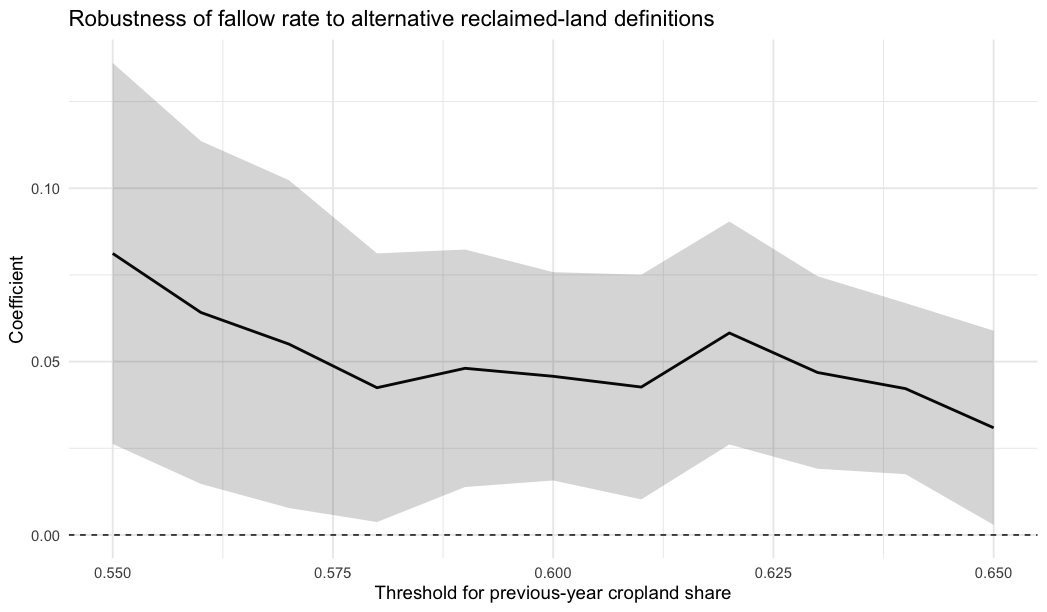
\includegraphics[width=\linewidth]{sensitivity_fallow_lowbound0.6.png}
        \caption{\footnotesize Fallow}
    \end{minipage}
    \hfill
    \begin{minipage}{0.48\linewidth}
        \centering
        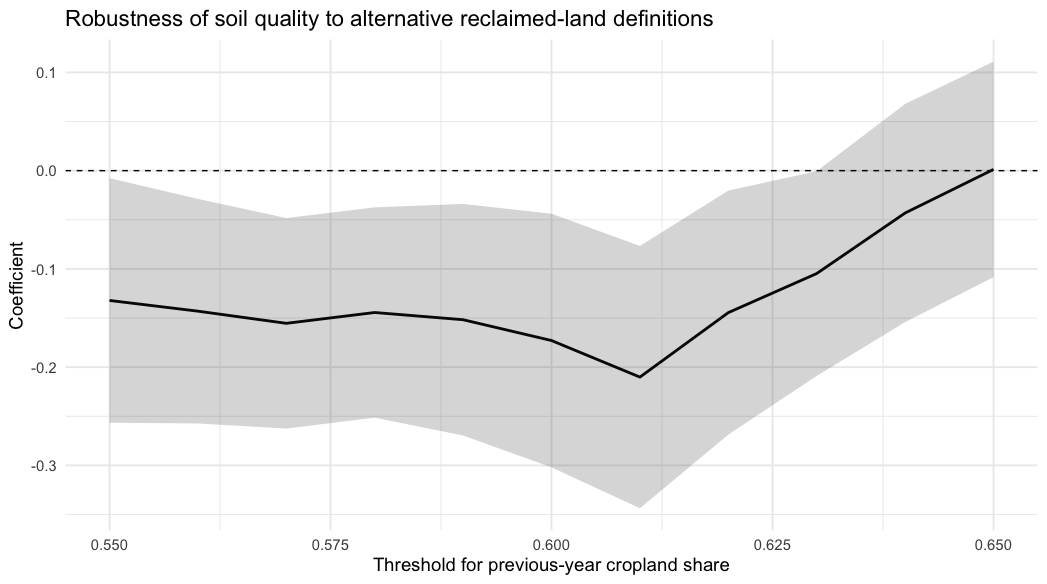
\includegraphics[width=\linewidth]{sensitivity_soil.png}
        \caption{\footnotesize Soil Quality}
    \end{minipage}
\end{figure}
\end{frame}

\begin{frame}{Sensitivity to Alternative Fallow Rate Definition}
    \begin{figure}
        \centering
        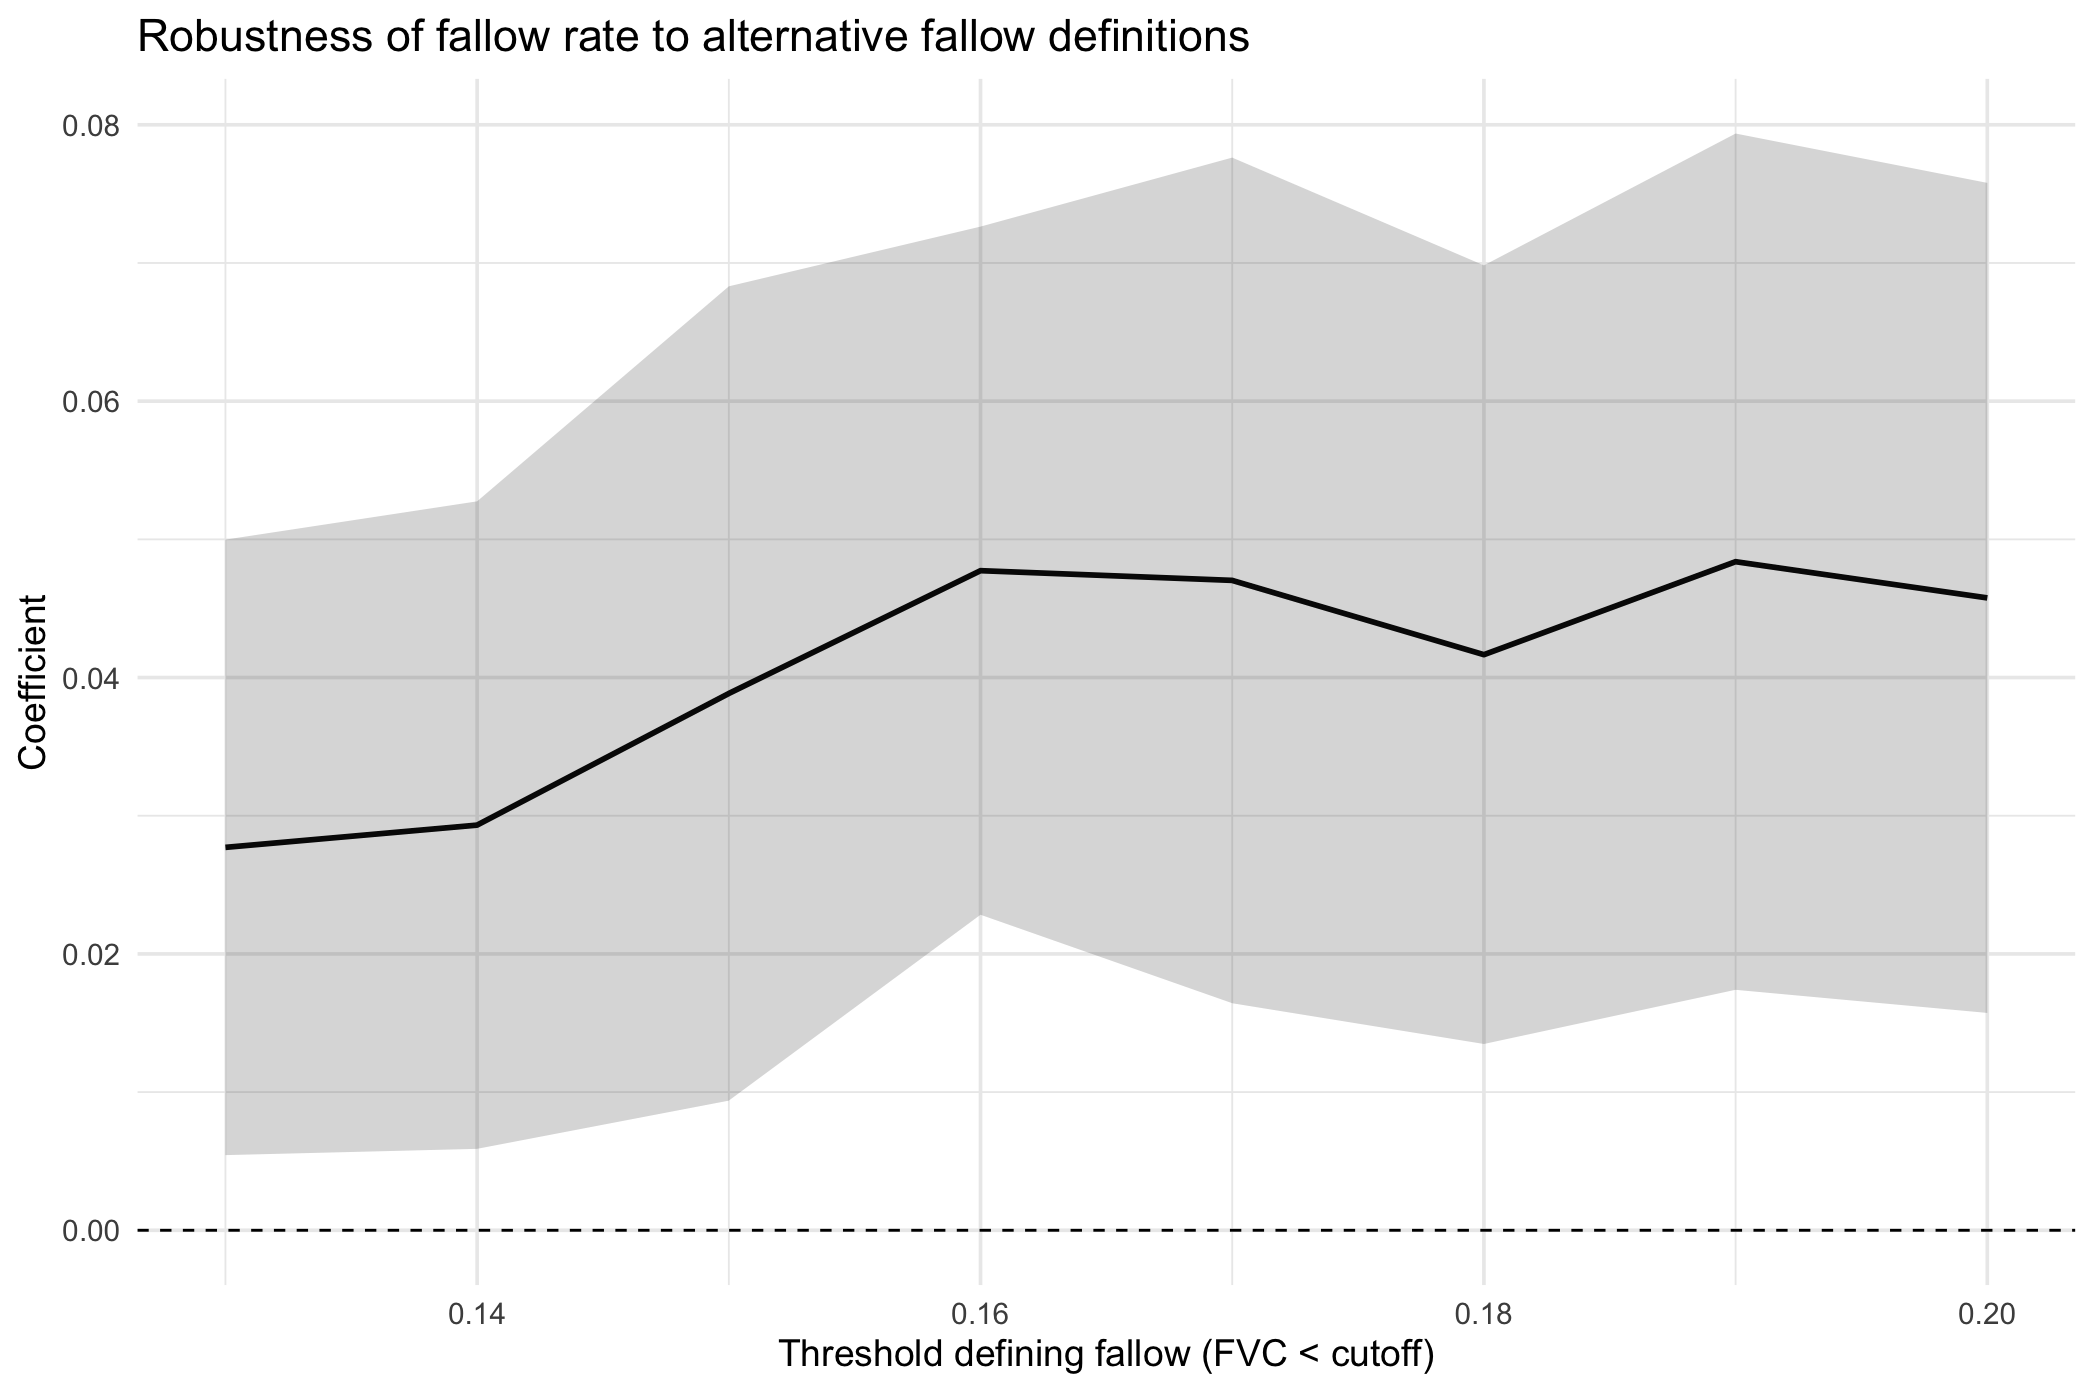
\includegraphics[width=0.7\linewidth]{sensitivity_fallow_rate0.2.png}
        \label{fig:placeholder}
    \end{figure}
\end{frame}


\bibliographystyle{aer}
\bibliography{literature}


\end{document}